\documentclass[preprint]{sigplanconf}

% The following \documentclass options may be useful:
%
% 10pt          To set in 10-point type instead of 9-point.
% 11pt          To set in 11-point type instead of 9-point.
% authoryear    To obtain author/year citation style instead of numeric.

\usepackage{amsmath}
\usepackage{graphicx}
\usepackage{url}
\usepackage{amssymb}
\usepackage{subfigure}
\usepackage{algorithm} 
\usepackage{algpseudocode}
\usepackage{epsfig}
\usepackage{fancyvrb}
%\usepackage{times}

% make an environment for subfigures with verbatim
\newbox\subfigbox	% Create a box to hold the subfigure. 
\makeatletter
  \newenvironment{subfloat}% % Create the new environment. 
    {\def\caption##1{\gdef\subcapsave{\relax##1}}%
    \let\subcapsave=\@empty % Save the subcaption text.  
    \let\sf@oldlabel=\label 
    \def\label##1{\xdef\sublabsave{\noexpand\label{##1}}}%
    \let\sublabsave\relax  %
    \setbox\subfigbox\hbox 
        \bgroup}% 
     {\egroup   %
    \let\label=\sf@oldlabel
    \subfigure[\subcapsave]{\box\subfigbox}}% 
\makeatother

\newcommand{\eightpoint}{\fontsize{8pt}{10pt}\selectfont}
\newcommand{\ninepoint}{\fontsize{9pt}{11pt}\selectfont}

%\advance \baselineskip by 0.4pt

% do not indent paragraphs of enumerated lists (my lists go on for pages...)
% numbers flush left to paragraph text: \leftmargin=17pt
\newcommand{\mybegin}{\begin{list}{\labelenumi}{\leftmargin=\parindent}\usecounter{enumi}}
\newcommand{\myitem}[1]{\item {\textit{\textbf{#1}}}}
%\newcommand{\myitem}[1]{\item {\bf #1}}
\newcommand{\myend}{\end{list}}
\newcommand{\mt}[1]{\mbox{\it #1}}
\newcommand{\todo}[1]{\framebox {\bf #1}}

\begin{document}

%\titlebanner{banner above paper title}        % These are ignored unless
%\preprintfooter{short description of paper}   % 'preprint' option specified.

\title{Representing and Parallelizing Induction Variable State in Stream Programs}

\authorinfo{Anonymous}
           {}
           {}

\maketitle

\begin{abstract}
As DSP programming is becoming more complex, there is an increasing
need for high-level abstractions that can be efficiently compiled.
Toward this end, we present a set of aggressive optimizations that
target linear sections of a stream program.  Our input language is
StreamIt, which represents programs as a hierarchical graph of
autonomous filters.  A filter is linear if each of its outputs can be
represented as an affine combination of its inputs.  Linear filters
are common in DSP applications; examples include FIR filters,
expanders, compressors, FFTs and DCTs.

We present a linear extraction analysis that automatically detects
linear filters based on the C-like code in their {\tt work} function.
Once linear filters are identified, we show how neighboring nodes can
be collapsed into a single linear representation, thereby eliminating
many redundant computations.  Also, we describe a method for
automatically translating linear nodes into the frequency domain,
thereby yielding algorithmic savings for convolutional filters.

We have completed a fully-automatic implementation of the above
techniques as part of the StreamIt compiler, and we demonstrate
performance improvements that average 400\% over our benchmark
applications.




\end{abstract}

%\category{CR-number}{subcategory}{third-level}

%\terms
%term1, term2

%\keywords
%keyword1, keyword2

\section{Introduction}

Applications that are structured around some notion of a ``stream''
are becoming increasingly important and widespread.  There is evidence
that streaming media applications are already consuming most of the
cycles on consumer machines \cite{Rix98}, and their use is continuing
to grow.  In the embedded domain, applications for hand-held
computers, cell phones, and DSP's are centered around a stream of
voice or video data.  The stream abstraction is also fundamental to
high-performance applications such as intelligent software routers,
cell phone base stations, and HDTV editing consoles.

Despite the prevalence of these applications, there is surprisingly
little language and compiler support for practical, large-scale stream
programming.  Of course, the notion of a stream as a programming
abstraction has been around for decades \cite{SICP}, and a number of
special-purpose stream languages have been designed (see
\cite{survey97} for a review).  Many of these languages and
representations are elegant and theoretically sound, but they often
lack features and are too inflexible to support straightforward
development of modern stream applications, or their implementations
are too inefficient to use in practice.  Consequently, most
programmers turn to general-purpose languages such as C or C++ to
implement stream programs.

There are two reasons that general-purpose languages are inadequate for
stream programming.  Firstly, they are a mismatch for the application
domain.  That is, they do not provide a natural or intuitive
representation of streams, thereby having a negative effect on
readability, robustness, and programmer productivity.  Moreover, because
the widespread parallelism and regular communication patterns of data
streams are left implicit in general-purpose languages, compilers are
not stream-conscious and do not perform stream-specific optimizations.
As a result, performance-critical loops are often hand-coded in a
low-level assembly language and must be re-implemented for each target
architecture.  This practice is labor-intensive, error-prone, and very
costly.

Secondly, general-purpose languages are a mismatch for the emerging
class of grid-based architectures \cite{smartmemories,rawshort,trips} that
are especially well-suited for stream processing.  Perhaps the primary
appeal of C is that it provides a ``common machine language'' for
von-Neumann architectures.  That is, it abstracts away the
idiosyncratic differences between machines, but encapsulates their
common properties: a single program counter, arithmetic operations,
and a monolithic memory.  However, for grid-based architectures, the
von-Neumann model no longer holds, as there are multiple instruction
streams and distributed memory banks.  Thus, C no longer serves as a
common machine language--in fact, it provides the wrong abstraction
for the underlying hardware, and architecture-specific directives are
often needed to obtain reasonable performance.  Again, this greatly
complicates the job of the programmer and hampers portability.

StreamIt is a language and compiler specifically designed for modern
stream programming.  The StreamIt language has two goals: first, to
provide high-level stream abstractions that improve programmer
productivity and program robustness within the streaming domain, and
second, to serve as a common machine language for grid-based
processors.  At the same time, the StreamIt compiler aims to perform
stream-specific optimizations to achieve the performance of an expert
programmer.

This paper motivates, describes, and justifies the high-level language
features of StreamIt, version 1.0.  The major limitation of StreamIt
1.0 is that all flow rates in the streams must be static; applications
such as compression that have dynamically varying flow rates will be
the subject of future work.  A large set of applications can be
implemented with static rates, and while dynamic rates will require a
different runtime model, it will still be essential to fully analyse
and optimize static sub-sections in order to obtain high performance.

The paper is organized as follows. In Section {\ref{sec:domain}}, we
characterize the domain of streaming programs that motivates the
design of StreamIt, and in Section~\ref{sec:overview} we describe the
language features in detail.  We present an in-depth example of a
software radio in Section~\ref{sec:example}, preliminary results in
Section~\ref{sec:results}, related work in Section~\ref{sec:related},
and conclusions in Section~\ref{sec:conc}.


%\begin{figure}[t]
%\eightpoint
%\begin{Verbatim}[numbers = left]
%int->int filter AssignPictureType(int width, 
%        int height, 
%        int numpictures) {
%    int frameno;
%
%    init {
%        frameno = 0;
%    }
%
%    work pop (width*height*3) push 2 {
%        push(frameno);
%        for (int i = 0; i < width*height*3; i++) {
%            pop();
%        }
%
%        int pushval;
%        int framecount = frameno % 12;
%        if (framecount == 0) {
%            pushval = 1;
%        } else if (framecount == 3 
%                || framecount == 6 
%                || framecount == 9) {
%            pushval = 2;
%        } else {
%            pushval = 3;
%        }
%
%        if ((frameno == (numpictures-1)) 
%            && (pushval == 3)) {
%            pushval = 2;
%        }
%
%        push(pushval);
%        frameno++;
%    }
%}
%\end{Verbatim}
%
%\caption{Example StreamIt program with AssignPictureType filter, used in MPEG Encoder.\protect\label{fig:apt-pipeline}}
%\end{figure}

\section{The StreamIt Language}
\label{sec:streamit}

StreamIt is an architecture-independent language for high-performance
stream programming~\cite{thies-cc02}.  The compiler is publicly
available~\cite{streamitweb} and includes backends for multicore
architectures, clusters of workstations, and Tilera architectures.

The model of computation in StreamIt is grounded in (but not limited
to) synchronous dataflow~\cite{lee87}.  In this model, the programmer
implements independent actors, or {\it filters}, which translate data
items from input channels to output channels.  Filters are composed
into graphs that represent the overall computation.  The key property
of synchronous dataflow is that the number of items consumed and
produced during each execution of a filter is known at compile time,
allowing the compiler to perform static scheduling and optimization.

An example StreamIt filter appears in Figure~\ref{fig:apt-pipeline}.
It is based on the AssignPictureType filter in the MPEG2 encoder.
StreamIt filters contain three stages of execution.  The most
important is the \work function, which represents the
steady-state execution step and is called repeatedly by the runtime
system.  Within the \work function, a filter may {\it peek} at a given
element on the input tape, {\it pop} an item off the input tape, or
{\it push} an item to the output tape.  The total number of items
peeked, popped, and pushed are declared as part of the \work function.
Note that if the peek rate exceeds the pop rate, it represents a
sliding window computation in which some input elements are accessed
across multiple invocations of the filter.

In addition to the \work function, a filter may declare an {\tt init}
function to initialize internal data structures, as well as a 
 \prework function (not given in Figure~\ref{fig:apt-pipeline}) to
perform specialized processing of data items prior to the steady
state.  The \prework function is needed in cases where the initial
processing has a different input or output rate than the steady-state
processing.

A {\it schedule} gives a multiplicity for each filter in a stream
graph.  The multiplicity indicates how often a filter's \work function
should be invoked (or \prework function on the first iteration of the filter).  The
{\it steady-state schedule} can be calculated such that all filters
fire in the schedule, and the schedule can be repeated
indefinitely~\cite{lee87}.  Steady-state execution of the graph
entails repeating the steady-state schedule for as much input as is
expected.  Execution of the stream graph is conceptually wrapped in an
outer loop that continuously executes the steady-state schedule.  All
the multiplicities of the steady-state can be multiplied by the same
constant $m$, and the result will still be a valid steady-state.  We
call this process {\it increasing} the steady-state of the graph by
$m$.

Furthermore, an {\it initialization} schedule enables the steady-state
schedule in the presence of peeking filters.  An initialization
schedule is required if peeking is present in a graph to enable the
calculation and execution of a steady-state
schedule~\cite{karczmarek-lctes03}.  During application execution, the
{\it init} function is called once for each filter, then the
initialization schedule is executed once, followed by an infinite
repetition of the steady-state schedule.

As depicted in Figure~\ref{fig:structures}, StreamIt provides three
hierarchical primitives for composing filters into stream graphs.  A
{\it pipeline} represents a sequential composition of streams, in
which the output of one stream feeds into the input of the next.  A
{\it splitjoin} represents a parallel set of streams, which divulge
from a common {\it splitter} and converge to a common {\it joiner}.
The types of splitters and joiners are predefined by the StreamIt
language; they encompass duplication and weighted round-robin
behaviors.  Finally, a {\it feedbackloop} represents a cycle in the
stream graph.

\begin{figure}[t!]
\centering
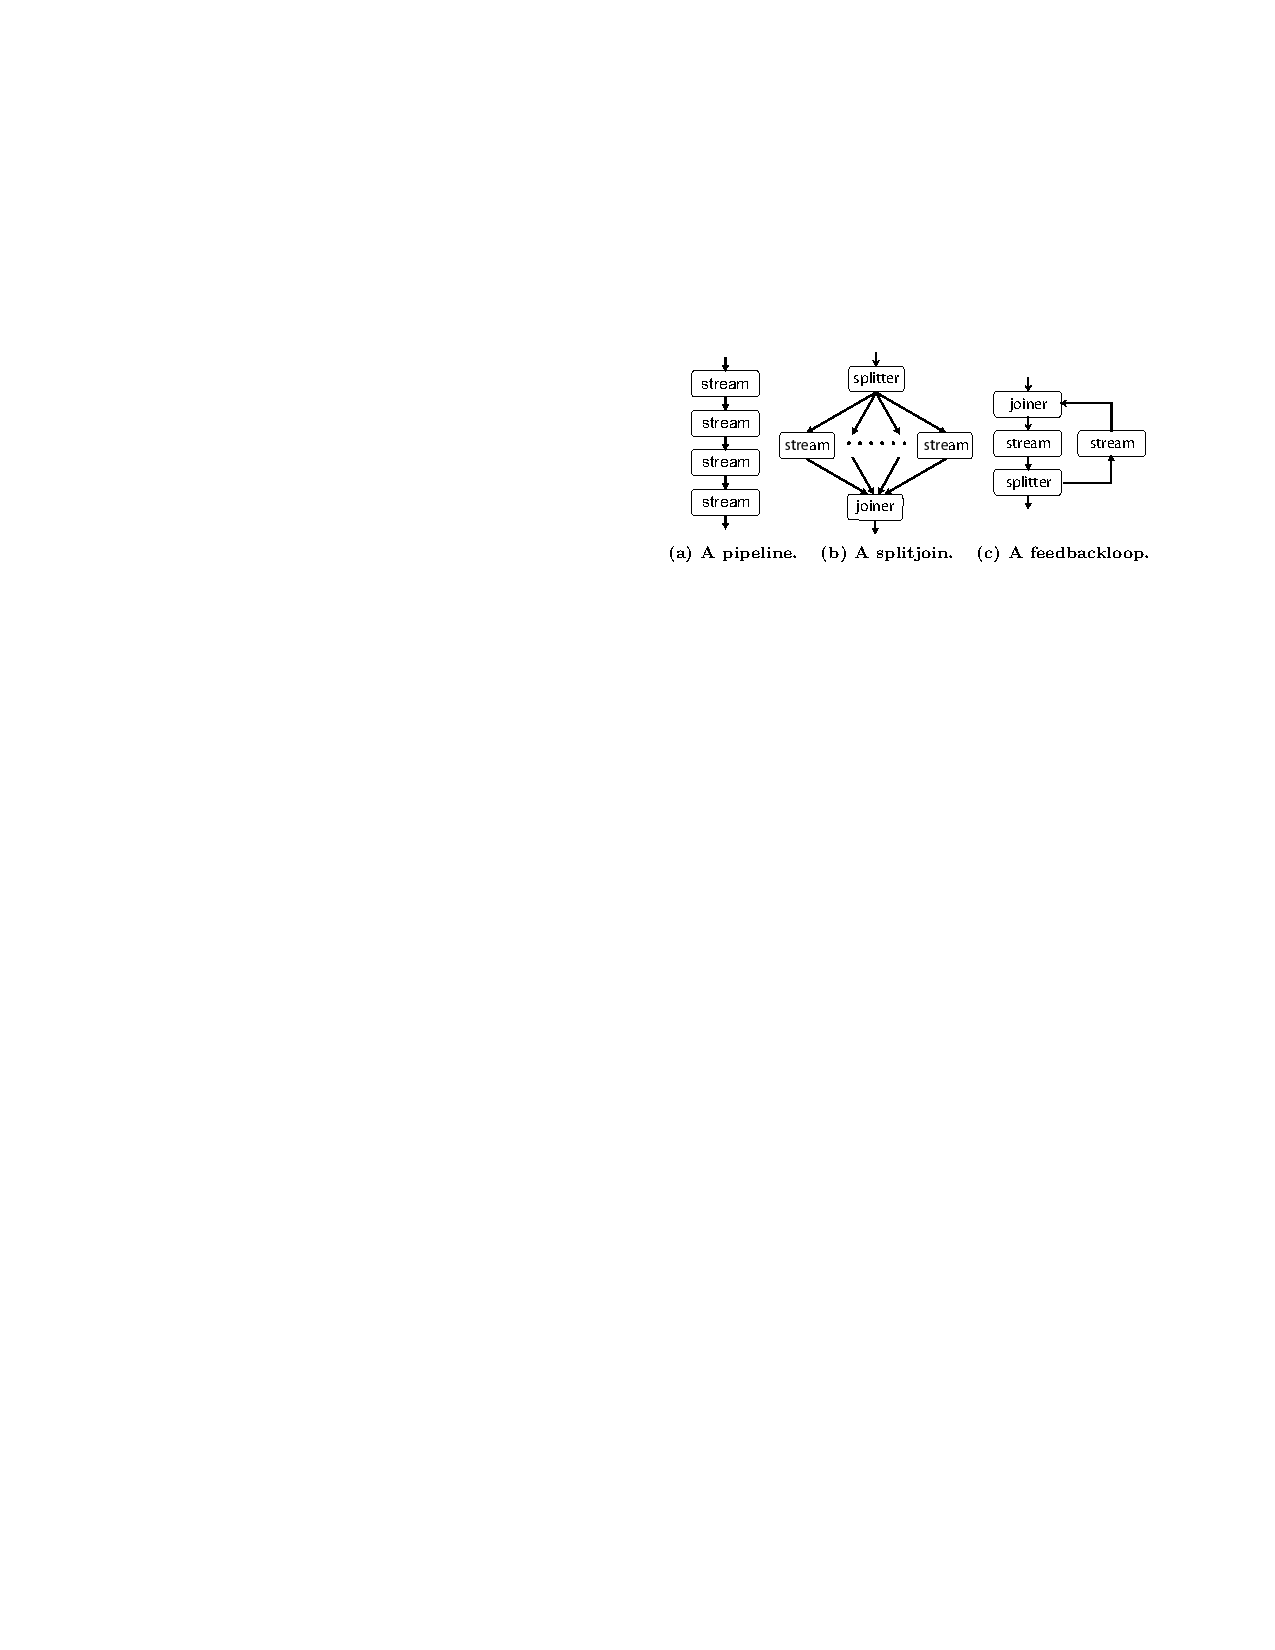
\includegraphics[width=3.3in]{stream-structures.pdf}
%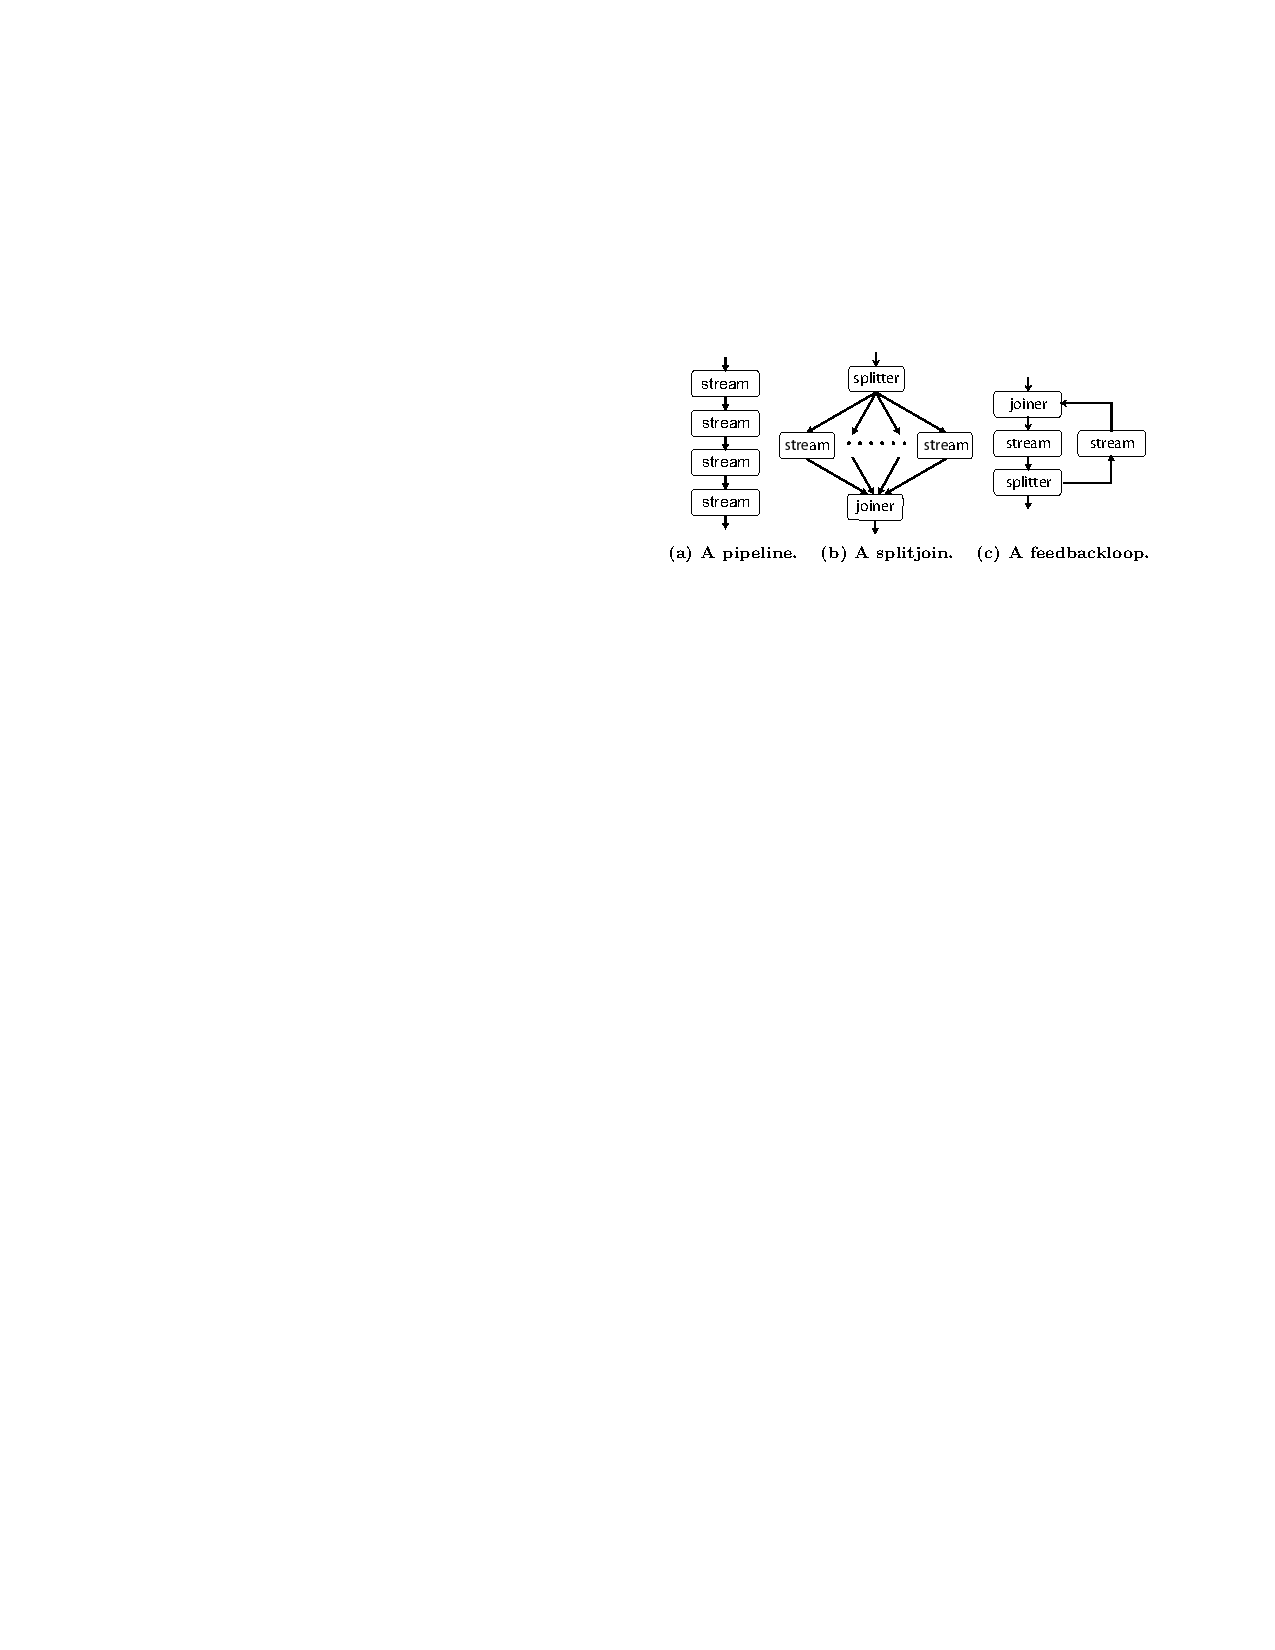
\psfig{file=stream-structures,width=\columnwidth}
\caption{Hierarchical stream structures supported by StreamIt.\protect\label{fig:structures}}
\end{figure}

The StreamIt compiler coarsens the granularity of a stream graph by
applying the {\it fusion} transformation which merges adjacent filters
into a single (large) filter (embedding the schedules of execution in
the merged filter)~\cite{streamit-asplos}.  The {\it fission}
transformation is employed to add data parallelism to a stream graph.
In fission, a single filter without state is duplicated a certain
number of ways and placed in a splitjion construct.  Input items to
the original filter are distributed among the duplicates, termed {\it
  fission products}.  In \S\ref{sec:fission}, we describe how to
extend the fundamental fission transformation to parallelize induction
variable state.

\section{Induction Variable State in Stream Programs}
\label{sec:inductionstate}

% \begin{figure}[t]
% {\eightpoint
% \begin{verbatim}
%   int->int stateful filter InductionFilter() {
%       int counter;
%       int max;
  
%       work push 1 pop 1{

%           ...

%           counter = (counter + 1);

%           if (counter > max) {
%               counter = 0;
%           } 
%       }
%   }
% \end{verbatim}
% \caption{Example of a stateful StreamIt filter using induction variable state.\protect\label{fig:filter-example}}}
% \end{figure}

Traditional induction variables encapsulate all variables that are
increased or decreased with iterations of a loop~\cite{Aho:1986, Fischer:2009}.  Induction variable
state as applied to stream programming is a class of state that
requires keeping count of how often a filter has been invoked.  Common
usage of induction variable state includes performing some special
action after a certain number of iterations and keeping track of array
index positions.  Many filters maintain multiple induction variables
as well, which may either be dependent or independent of each other.

Many applications in the StreamIt benchmark suite, including MPEG2 encoder,
Medium Pulse Doppler, Trellis, and FIRBank (pipelined version), maintain induction variable state 
by creating a mutable state field in the corresponding filter.  This
state can be set to the desired starting value.  The induction
variable is consistently updated at some point during the work call.
For many use cases, this induction variable may need to be reset if it
reaches a certain threshold. 

Figure~\ref{fig:apt-pipeline} illustrates a common pattern of explicit
induction variable state.  It is based on the AssignPictureType filter in 
the MPEG2 encoder. The implementation of the filter maintains
a filter variable {\tt frameno} that is incremented on each call of
the {\tt AssignPictureType}'s work function.  This variable
represents state.  Each iteration of the 
filter uses a value for {\it frameno} dependent on what the value of
{\it frameno} was in the previous iteration.  The {\tt framecount} variable is derived
from this state and used in control flow.

As presently constructed, induction variable state for\-ces the
corresponding filter to be run in sequential order.  In providing a
mutable state whose value is dependent on the previous execution step,
it is necessary to run a filter execution step and establish the
induction variable value before moving on to the next execution step.
The tradition fission transformation would not be able to parallelize
this filter without understanding how to properly distribute the
calculation of the state.  As such, it is not possible 
to create duplicates and run them in a parallel fashion.  

With induction variable state, it is possible to make the 
compiler aware of such state through the keyword solution.  
Figure~\ref{fig:apt-pipeline} shows how the same AssignPictureType filter can be 
rewritten to use the keyword.  The compiler can generate the value
for {\tt iter()} for each iteration of the AssignPictureType filter independent
of previous iterations.  Duplicates of the filter can be made and
data parallelism opportunities can be exploited.


\subsection{Scalability Implications of Eliminating Induction Variable State}
\label{sec:model-analysis}
Table~\ref{fig:benchmarks} indicates programs in the StreamIt benchmark suite that use induction variable filters (not including source filters) in the manner described above.  The StreamIt compiler provides static estimations of work performed in filters.  The above table indicates the work performed in specifically the induction variable filters.

The majority of programs do not have substantial work performed in filters using induction variables; FIRBankPipeline and MPD contain only a few stateful filters whose total work concentration is fairly low.  The MPEG-2 motion estimation subset is the only exception because its stream graph is comprised mostly with stateful filters.  However, eliminating any form of state will have a large impact on runtime performance even on programs with low work concentration in stateful filters.  We model the potential speedups of a particular stateful program in this subsection.  For the purpose of this analysis, we will assume no communication cost between filters.  We will also assume the compiler exposes no pipeline parallelism.  This assumption forces the serialization of stateful filters on the stream graph.

\begin{table}[t]
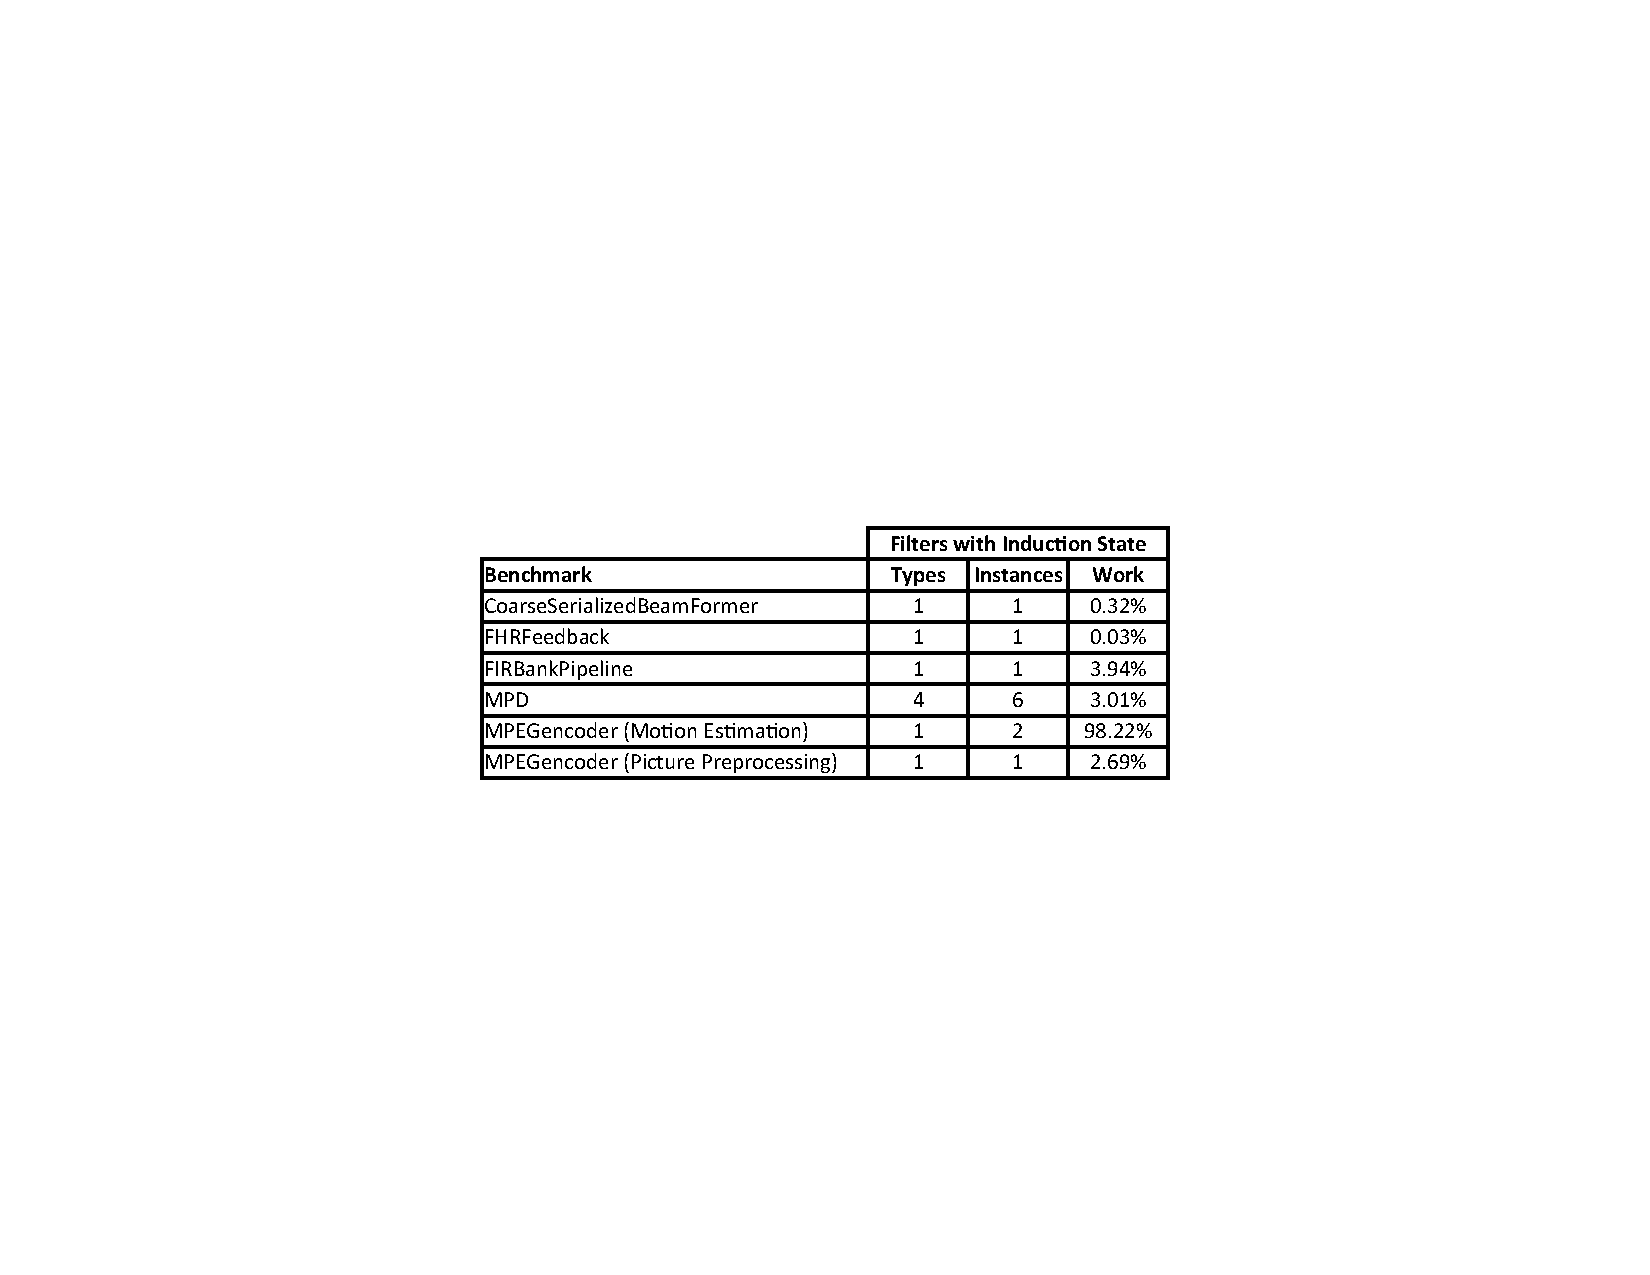
\includegraphics[width=3.3in]{figures/induction-benchmarks.pdf}
\caption{Benchmarks using induction variable state and estimations on work performed in filters with induction state.\protect\label{fig:benchmarks}}
\end{table}

Let $N$ be the number of cores we are planning to parallelize over.  Let $\sigma$ be the percentage of work performed in stateful filters that can have its state eliminated, in this case solely filters that use induction variable state.  

If $\sigma = 0$, the entire program is stateless.  The program can be fused to coarsen the granularity, then fissed and mapped to all of the available cores.  Each core would perform $\frac{1}{N}$ of the total work.  Thus with no state, the program can exhibit speedups of up to $N$ times the single-core runtime.

For filters that contain stateful work, $1-\sigma$ of the work in the program is considered stateless, and thus can be fissed and assigned to $N$ individual cores.  The stateful filters cannot be parallelized, and is sequential to all work in the program.  The total serialized work is $\frac{1-\sigma}{N} + \sigma$.  Thus the total speedup is the serial work divided by the new parallelized work.  
\begin{eqnarray*}
\dfrac{1}{\frac{1-\sigma}{N} + \sigma} &=& \dfrac{N}{1 + \sigma(N-1)}
\end{eqnarray*}

We can characterize the amount of speedup between a completely stateless program to an equivalent stateful program with $\sigma$ percentage of stateful work.  This is simply:
\begin{eqnarray*}
\dfrac{N}{\frac{N}{1 + \sigma(N-1)}} &=& 1 + \sigma(N-1)
\end{eqnarray*}

\begin{figure}[t!]
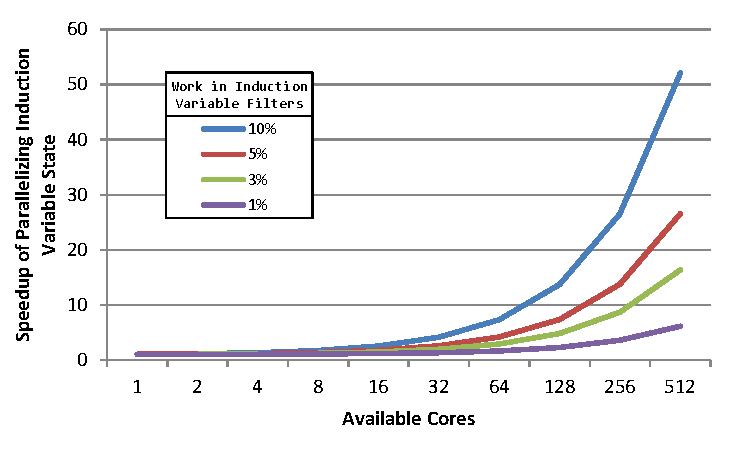
\includegraphics[width=3.3in]{figures/theoretic-speedup.pdf}
\caption{Theoretical speedups of stateless programs over corresponding stateful programs with $\sigma$\% work in filters using induction variable state.  \protect\label{fig:theo-speedups}}
\end{figure}

Figure~\ref{fig:theo-speedups} indicates the potential speedups over stateful programs given stateful work percentages and a varying number of cores.  Even benchmarks in the suite that exhibit only 3\% work in stateful filters can exhibit 8x speedups with 256 cores.  Providing a means to remove state from filters that exhibit very small amounts of work relative to the rest of the program can still generate substantial speedups in the near future.


\section{Iteration Keyword}

The stream programming paradigm allows the burden of induction variable state to be shifted from the programmer to the compiler.  With the introduction of a new language construct, hereafter referred to as {\tt iter()}, the programmer can take measures to write their programs with data parallelism in mind.  Use of {\tt iter()} potentially provides further benefits in programmability and code readability as well.

As described before, induction variable state requires the user to maintain mutable state, updating such state within the filter invocation, and potentially resetting them when required.  In providing the {\tt iter()} keyword, the programmer can eliminate much of this code simply by arithmetically manipulating {\tt iter()} usage.  

[examples for single induction variable elimination, multiple nested induction variable elimination, varying starting values]

The transformation from filters using induction variable state to using {\tt iter()} is fairly simple for users to implement.  Many of these transformations follow the same approach as induction variable elimination.  The induction variable can be expressed as an arithmetic manipulation of {\tt iter()}.

In having the user define their induction variables using {\tt iter()}, it is possible to eliminate code required to reset or update the induction value.  For large filters, the maintenance of this state may be difficult to follow.  The approach illustrated in the examples shows how it is possible to remove much of the code required to maintain this state with the {\tt iter()} keyword.  

For filters that define multiple induction variables, it is possible to redefine these values in terms of {\tt iter()} as well.  It is not necessary to maintain multiple separate values for state.  Independent and nested induction variable state alike can be defined with use of {\tt iter()}.

This approach of using {\tt iter} to define induction variable state helps users to write filters in a stateless manner.  The user can think about programming their filters in a stateless manner, and thereby exposing data parallelism. 



\section{Design Rationale}

Our approach in removing induction variable state is to introduce a new language construct.  The language construct maintains a value indicating how often the corresponding filter has been invoked.  This approach was chosen over implementing a system to automatically recognize induction variable usage in filter construction.

The approach of automatic analysis would require looking for an induction variable defined in the filter.  The simplest form of this analysis would require first idiomatically detecting for a variable modified by a statement similar to \texttt{var = var + 1}.  Very few iteration filters (outside of source filters) use induction state in this limited capacity.  Consider Figure~\ref{fig:weight-calc}, where the induction variable is incremented at each iteration step, until a certain threshold value at which it will reset.  This pattern is very common in programs that use induction filters.  MPD and FIRBank use this technique to iterate across a provided array one element per iteration step.  To ensure consistency between iteration steps, the automatic analysis is required to detect these types of updates as well.  

\begin{figure}[t]
{\eightpoint
\begin{verbatim}
float->float stateful filter WeightCalc(int n)
{
  float[n] window;
  int windowPos;

  ...

  // the input stream is multiplied with the weights
  work push 2 pop 2
  {

    push(pop() * window[windowPos]);
    push(pop() * window[windowPos]);

    windowPos++;
    if(windowPos >= n)
    {
      windowPos = 0;
    }
  }
}
\end{verbatim}
\caption{MPD filter that multiplies stream values with weights.\protect\label{fig:weight-calc}}}
\end{figure}

\begin{figure}[t]
{\eightpoint
\begin{verbatim}
float->float stateful filter CFARDetectFilter(int rows, int cols)
{
  int currentCol;
  int currentRow;

    ...

  work pop 3 push 1
  {
      ...

    currentRow++;
    if(currentRow >= rows)
    {
      currentRow = 0;

      currentCol++;
      if(currentCol >= cols)
      {
        currentCol = 0;
      }
    }
  }
}
\end{verbatim}
\caption{MPD CFAR Detect filter.\protect\label{fig:cfar-detect-filter}}}
\end{figure}

A filter may have multiple induction variables that are dependent on one another in defining their values.  Consider Figure~\ref{fig:cfar-detect-filter}, a filter used in MPD maintaining nested induction variables.  The automatic analysis must also be able to detect incrementing statements that may not necessarily be updated on every work call.  The process of simply detecting and identifying induction variables can potentially branch into many cases that need to be specially implemented.

There may potentially be other special cases that must be defined into the automatic analysis.  Filters may have also define induction variables to start with and reset to a particular value.  Induction variables may increment by a different value other than 1 at each execution step.  Though the methods of using induction variables as illustrated in Figure~\ref{fig:cfar-detect-filter} and Figure~\ref{fig:weight-calc} encompass many of the common use cases in the benchmark suite, slight variations in the implementation to the pattern may prevent the induction variable from being detected.

Accordingly, there are several downsides to the approach of automatic analysis.  Automatic recognition is a fairly inflexible process in detecting induction variable state.  As illustrated, there may be many different ways of defining induction variables.  Nested counters are often used to track row and column indexes in two-dimensional arrays.  Co-induction variables may be constructed to reset the value of other variables after reaching a certain value.  The many different uses of induction variables may be difficult to assess.  Automatic recognition would restrict data parallelism opportunities to only the filters that fit the implemented templates.  We instead elect to provide the user with the flexibility of defining derived induction values while providing parallelism opportunities.  

The keyword solution also has the added benefit of maintaining a value that is predictable in its updates.  The value that the keyword returns is simply the current iteration number for that the corresponding filter has run.  This is a value that always increments by one at the end of every work call.  Automatic recognition is a frail process because it is difficult to predict how the induction value will be updated, as illustrated in the above figures.  

The approach of automatic analysis also does little to encourage programming with parallelism in mind.  User written code will still maintain state, which inhibits data parallelism opportunities.  In introducing a language construct, user written code eliminates explicitly kept state.  This approach encourages users to write code with the intention of exploiting parallelism.



\subsection{Comparison to Coarsening}
\label{sec:coarsen}

% \begin{figure}[t]
% {\eightpoint
% \begin{verbatim}
% float->float stateful filter WeightCalc(int n)
% {
%   float[n] window;
%   int windowPos;

%   ...

%   // the input stream is multiplied with the weights
%   work push 2 pop 2
%   {

%     push(pop() * window[windowPos]);
%     push(pop() * window[windowPos]);

%     windowPos++;
%     if(windowPos >= n)
%     {
%       windowPos = 0;
%     }
%   }
% }
% \end{verbatim}
% \caption{MPD filter that multiplies stream values with weights.\protect\label{fig:weight-calc}}}
% \end{figure}

In cases of explicit induction variable state where the induction
variable is reset after a certain number of iterations, the filter can
be converted into a stateless filter by {\it coarsening} the filter,
increasing the number of input items that are required for the work
function execution.  Figure~\ref{fig:wc-example}(a) lists the weight
calculation filter from the Medium Pulse Doppler (MPD) benchmark.  The
filter includes explicit induction variable state as originally
implemented by the programmer.  This filter can be rewritten without
state (and without using the {\tt iter()} keyword) by coarsening the
filter such that each work function execution operates on a larger
subset of the input.  Figure~\ref{fig:wc-example}(b) lists a coarsened
implementation that is stateless.  In the coarsened implementation the
filter requires $2n$ input items.

Figure~\ref{fig:wc-example}(c) lists the implementation of the weights
calculation filter utilizing the {\tt iter()} keyword.  Notice that
the filter operates at a finer granularity versus the coarsened
version and that it operates at the same granularity as the original
filter.  Although the {\tt iter()} implementation includes a modulo
operation per output, calculation of outputs will be parallelized
(see Section~\ref{sec:fission}).

The mantra of stream programming is that the programmer should not be
burdened with parallelization, granularity, communication or
synchronization concerns.  Implementing a filter at a fine granularity
allows the compiler or runtime to decide on the best granularity for a
given architectural target.  In practice the use of the {\tt iter()}
keyword is preferred over a coarsening conversion because:

\begin{itemize}

\item The programmer grasped the algorithm and implemented the
  application at the fine granularity.  A language should constrain
  the programmer as little as possible for the sake of performance.

\item The coarse granularity implementation requires larger input and
output buffers to implement because of the larger push and pop rates.
Larger buffers occupy more of the cache and could evict filter data or
instructions are needed during execution.  Thus there could be more
accesses to longer latency memory hierarchies~\cite{sermulins-lctes05}.

\item Larger input and output rates also interact with the
  steady-state scheduling algorithm.  Since the scheduling algorithm
  is performing many cascading LCMs, a single filter with large input
  and output rates will increase the multiplies of all filters of the
  application, requiring more buffering and increasing
  latency~\cite{karczmarek-lctes03}.  The use of the {\tt iter()}
  keyword does not force the programmer to sacrifice latency for
  parallelization.

\end{itemize}


\newcommand{\entry}[1]{\raisebox{0pt}[24pt][20pt]{\parbox{2.75in}{#1}}}
\newcommand{\entrymed}[1]{\raisebox{0pt}[36pt][30pt]{\parbox{2.75in}{#1}}}
\newcommand{\entrybig}[1]{\raisebox{0pt}[42pt][36pt]{\parbox{2.75in}{#1}}}

This section walks through a sample session with the compiler and
runtime system.  We will use the {\tt FMRadio} example from the
StreamIt release as a running example.  To get started, change to the
following directory:
{\small
\begin{verbatim}
% cd $STREAMIT_HOME/apps/examples/cookbook
\end{verbatim}
}
\noindent The example is in {\tt FMRadio.str}. The following
sections describe the compilation of {\tt FMRadio} using the
uniprocessor backend, the Java library, and the Raw backend.  A
summary of the compiler's command-line options can be found in
Appendix~\ref{ap:options}, or by typing {\tt strc -help} at the
command line.

\subsection{Compiling for a Uniprocessor}

There are two ways to compile a StreamIt program for execution on a
general-purpose processor.  Both methods compile StreamIt to a C
program that can be further compiled with a C compiler.  The first
method (the default) preserves the hierarchical structure of the
original program and relies on a C runtime library to do buffer
management.  The second method (``standalone'') produces a
self-contained file where the entire stream graph has been collapsed
into a single function, with buffer management embedded into the code.
The default output is more readable and provides some flexibility (by
exposing the runtime library interface).  The standalone output might
be useful for groups interested in compiling C programs to new
architectures; however, the size of the main work function might grow
very large.  We recommend using the default backend with the C runtime
library.

\medskip {\bf Compiling for C library.}  To compile {\tt FMRadio} using the
uniprocessor backend and C runtime library, issue the following
command (the compiler output is shown): {\small
\begin{verbatim}
% strc FMRadio.str -o fm
Running Constant Prop and Unroll... done.
Raising variable declarations... done.
Propagating constant fields... done.
Flattening blocks... done.
Raising variables... done.
Raising variable declarations... done.
Moving initial assignments... done.
Structuring... done.
Scheduling... got schedule, interpreting... done.
Annotating IR for uniprocessor... done.
Generating code...
\end{verbatim}
} 
This will create a C file named FMRadio.c and a binary named {\tt
fm}.  The binary can be executed for 5 steady-state iterations as follows:
{\small
\begin{verbatim}
% ./fm -i 5
278074.000000
278074.750000
278075.437500
278075.968750
278076.437500
\end{verbatim}
} 
During the compilation process, several {\tt dot} graphs are
generated.  The {\tt dot} format can be displayed and converted to
other formats using the Graphviz software, which is available
online\footnote{\tt http://www.research.att.com/sw/tools/graphviz/}.
For example, we can examine a stream graph for the FM application as
follows: {\small
\begin{verbatim}
% dotty first-sir-tree.dot
\end{verbatim}
} The result appears in Figure~\ref{fig:fm-sir-tree}.  A complete list
of the {\tt dot} graphs that are produced on the normal uniprocessor path
are shown in Figure~\ref{fig:dot-uni}.

\begin{figure}[t]
\hspace{-0.75in}\psfig{figure=fm-sir-tree.eps,width=6.6in}
\caption{{\tt first-sir-tree.dot} for the FMRadio example.\protect\label{fig:fm-sir-tree}}
\end{figure}

\begin{figure}[t]
{\small
\noindent \begin{tabular}{|l|l|}
\hline
{\bf Filename} & {\bf Description} \\
\hline
{\tt first-sir-tree.dot} & \entry{Original stream graph, as written by programmer.} \\ \hline
{\tt before-partition.dot} & \entry{Canonical version of stream graph, before any stream transformations are applied.  Nodes are annotated with their I/O rates.}\\ \hline
{\tt after-partition.dot} & \entry{Canonical version of stream graph, after any stream transformations are applied.  Nodes are annotated with their I/O rates.}\\ \hline
{\tt schedule.dot} & \entry{Final stream graph, annotated with I/O rates and the number of times each node executes in the initial and steady-state schedule.} \\ \hline
\end{tabular}
}
\caption{{\tt dot} graphs produced on the uniprocessor path.\protect\label{fig:dot-uni}}
\end{figure}

\medskip {\bf Domain-specific optimizations.}  It turns out that our
version of the FMRadio has a lot of redundant computation the way in
which it is written.  For example, each {\tt BandPassFilter} could be
implemented as a single FIR filter rather than a composition of {\tt
LowPassFilter}'s; in fact, the entire equalizer could be collapsed to
a single FIR filter.  Further, some of these operations are more
efficient if executed in the frequency domain, with an FFT/IFFT being
used to translate to and from the time domain.

The StreamIt compiler includes a set of domain-specific optimizations
that will automatically perform the transformations described above.
The analysis considers all filters that are ``linear''---that is, each
of their outputs is an affine combination of their inputs.  The
compiler automatically detects linear filters by analyzing the code in
their work functions.  Then, it performs algebraic simplification of
adjacent linear filters, as well as automatic translation to the
frequency domain.  Since these transformations can sometimes hamper
performance, the compiler also does a global cost/benefit analysis to
determine the best set of transformations for a given stream graph.

\begin{figure}[t]
\hspace{3pt} \psfig{figure=fm-linear-simple.eps,width=4.6in}
\caption{{\tt linear-simple.dot}, which illustrates the linear sections of FMRadio.  Linear filters are shaded blue, while linear containers are shaded pink.\protect\label{fig:fm-linear-simple}}
\end{figure}

\begin{figure}[t]
\vspace{-6pt}
\begin{center}
\mbox{}\psfig{figure=fm-after-linear.eps,width=2.5in}
\vspace{-6pt}
\caption{Final stream graph ({\tt after-linear.dot}) for the FMRadio, compiling with the {\tt -linearpartition} option.\protect\label{fig:fm-after-linear}}
\end{center}
\vspace{-14pt}
\end{figure}

The {\tt linearpartition} option to strc will enable linear analysis
and optimizations\footnote{In contrast, the {\tt linearreplacement}
and {\tt frequencyreplacement} options will perform maximal algebraic
simplification and frequency translation, respectively, even in cases
where it is not beneficial.}:
{\small
\begin{verbatim}
% strc -linearpartition FMRadio.str -o fm
Running Constant Prop and Unroll... done.
Raising variable declarations... done.
Propagating constant fields... done.
Flattening blocks... done.
Raising variables... done.
Raising variable declarations... done.
Moving initial assignments... done.
Running linear analysis...
WARNING: Assuming method call expression non linear(atan). Also 
  removing all field mappings.
WARNING: Insufficient pushes detected in filter
done with linear analysis.
Linear partitioner took 1 secs to calculate partitions.
Structuring... done.
Scheduling... got schedule, interpreting... done.
Annotating IR for uniprocessor... done.
Generating code...
\end{verbatim}
} 
%
The linear analysis produces its own set of {\tt dot} files that we
can use to inspect the results of the optimizations.  For example, the
following command will display the stream graph with the linear
sections highlighted: {\small
\begin{verbatim}
% dotty linear-simple.dot
\end{verbatim}
} 
%
As shown in Figure~\ref{fig:fm-linear-simple}, FMRadio contains many
linear components, including the first LowPassFilter and the
equalizer.  To see the stream graph after linear optimizations have
been applied, we can issue the following command:
{\small
\begin{verbatim}
% dotty after-linear.dot
\end{verbatim}
} 
%
As illustrated in Figure~\ref{fig:fm-after-linear}, this stream
graph shows that the equalizer was collapsed into a single filter and
then was translated to the frequency domain (by virtue of the ``Freq''
prefix in the filter's name.)  However, the LowPassFilter at the top
was left unmodified; this is because it has a large pop rate that
degrades the performance of the frequency transformation.  In this
case, the linear optimizations lead to a 6.5X improvement in
throughput.

The linear optimizations produce additional {\tt dot} graphs; see
Figure~\ref{fig:dot-linear} for details.  For more information on the
linear analysis and optimization, please refer to {\tt http://cag.lcs.mit.edu/linear}.

\begin{figure}[t]
\vspace{-6pt}
{\small
\noindent \begin{tabular}{|l|l|}
\hline
{\bf Filename} & {\bf Description} \\
\hline
{\tt ldp-partition-input.dot} & \entry{The stream graph as it was input to the linear partitioning algorithm.}\\ \hline
{\tt linear.dot} & \entry{The stream graph with linear filters highlighted and each node annotated with its I/O rates.}\\ \hline
{\tt linear-simple.dot} & \entry{Same as {\tt linear.dot} but without the I/O rates.}\\ \hline
{\tt after-linear.dot} & \entry{The stream graph after linear transformations are complete.} \\ \hline
\end{tabular}
}
\vspace{-5pt}
\caption{{\tt dot} graphs produced by linear optimizations.\protect\label{fig:dot-linear}}
\vspace{-5pt}
\end{figure}

\bigskip {\bf Compiling as standalone.}  To compile FMRadio to a
standalone file that can execute without the C runtime library, use
the {\tt -standalone} option:
{\small
\begin{verbatim}
% strc -standalone FMRadio.str -o fm
/*
Out of Kopi2SIR.
Out of semantic checker.
*/
Entry to RAW Backend
Moving initializers into init functions... done.
Running Constant Prop and Unroll...
Done Constant Prop and Unroll...
Running Constant Field Propagation...
Done Constant Field Propagation...
Running Partitioning...
  Found 26 tiles.
  Building stream config...
  Calculating partition info...
  Tracing back...
  Work Estimates:
    Fused_Flo_Low_FMD_Low_Pre_E...      10240   (100%)
Done Partitioning...
Flattener Begin...
Filters in Graph: 1
Flattener End.
Simulated Annealing Assignment
Tiles layout.assigned: 1
Initial Cost: 0.0
Assign End.
Switch Code Begin...
FineGrainSimulator Running...
End of init simulation
End of steady-state simulation
sw0.s written
Switch Code End.
Generating Raw Code: 
  Fused_Flo_Low_FMD_Low_Pre_EqS_Pos_Fil_Flo_172 (no buffer)
Tile Code begin...
Optimizing Fused_Flo_Low_FMD_Low_Pre_EqS_Pos_Fil_Flo_172...
Code for Fused_Flo_Low_FMD_Low_Pre_EqS_Pos_Fil_Flo_172 
  written to tile0.c
Tile Code End.
Creating Makefile.
Exiting
\end{verbatim}
} 
%
As is evident in the compiler output above, the standalone option
utilizes the Raw backend and stores the self-contained output file in
{\tt tile0.c} (as well as the binary {\tt fm}).  Also, due to an
implementation detail, it is not possible to control the number of
runtime iterations for standalone programs (they will run forever.)

\subsection{Using the Java Library}

A convenient aspect of the StreamIt compilation toolchain is that all
StreamIt programs are first translated to Java files that can be
executed against a Java runtime library using a normal Java Virtual
Machine.  This is especially useful for testing and debugging
applications, as well as validating the output of the compiler.

The library can be invoked with the {\tt -library} flag.  Since {\tt
strc} will both compile and execute the file in the library, you can
specify the number of iterations to execute with the {\tt -i} flag.
For example, to compile FMRadio and run for 5 iterations in the
library, do as follows\footnote{In this case, the library's output is
marginally different from the compiler's due to numerical precision
issues.}:
%
{\small
\begin{verbatim}
% strc -library -i 5 FMRadio.str
278073.94
278074.75
278075.38
278075.94
278076.4
\end{verbatim}
} 
%
You can also inspect the {\tt FMRadio.java} file, which was generated
for execution in the library.  It can be compiled and run with a
standard Java compiler and JVM.  The library also produces a {\tt dot}
graph of the program; it is given the same name as the StreamIt file,
but with a {\tt dot} extension ({\it i.e.,} it is {\tt FMRadio.dot} in
this case.)

There are a few additional options available in the library.  For
instance, you can direct the library not to execute the program, but
to instead just print the schedule of filter firings:
{\small
\begin{verbatim}
% strc -library -norun -printsched FMRadio.str
init = [
$0 = FloatOneSource@3541984.work
$1 = LowPassFilter@4565111.work
$2 = FMDemodulator@1233730.work
$3 = EqSplit@4689495.duplicate
$4 = BPFCore@6288523.duplicate
$5 = BPFCore@4074853.duplicate
$6 = BPFCore@5058143.duplicate
$7 = BPFCore@2951274.duplicate
$8 = { {379 $0} {64 $1} {63 $2} {63 $3} 
       {63 $4} {63 $5} {63 $6} {63 $7} }
]
steady = [
$9 = LowPassFilter@3738425.work
$10 = LowPassFilter@1042371.work
$11 = BPFCore@6288523.roundrobin
$12 = Subtracter@3144816.work
$13 = EqSplit$2@6700605.work
$14 = LowPassFilter@5188736.work
$15 = LowPassFilter@7510100.work
$16 = BPFCore@4074853.roundrobin
$17 = Subtracter@1467553.work
$18 = EqSplit$2@2671847.work
$19 = LowPassFilter@503498.work
$20 = LowPassFilter@6589979.work
$21 = BPFCore@5058143.roundrobin
$22 = Subtracter@2069821.work
$23 = EqSplit$2@8316668.work
$24 = LowPassFilter@1649037.work
$25 = LowPassFilter@7808535.work
$26 = BPFCore@2951274.roundrobin
$27 = Subtracter@230849.work
$28 = EqSplit$2@4354460.work
$29 = EqSplit@4689495.roundrobin
$30 = Equalizer$1@3615258.work
$31 = FloatPrinter@2964388.work
$32 = { {5 $0} $1 $2 $3 $4 $9 $10 $11 $12 $13 $5 $14 $15 $16 $17 $18
        $6 $19 $20 $21 $22 $23 $7 $24 $25 $26 $27 $28 $29 $30 $31 }
]
!ml sched size = 39
!ml buff size = 1299
\end{verbatim}
%$
} 
%
Currently, the default scheduler is a minimal latency scheduler that
uses phases to compress the code size.  The schedule listed above has
two components: an initialization schedule (to initialize buffers for
filters that peek) and a steady-state schedule (that can loop
infinitely).  Each filter and splitter in the graph is given a number
for easy reference, and then the schedule is printed at the bottom.  A
loop nest in the schedule is denoted by {\tt (N F)}, where the filter
{\tt F} executes {\tt N} times.  The schedule size and buffer size
required are printed at the end of the listing.

Additional options for the library can be found in
Appendix~\ref{ap:options}.

\subsection{Compiling for Raw}

To compile for an {\tt NxN} Raw machine, use the {\tt -raw N}
option\footnote{You can also compile for an NxM machine by using {\tt
-raw N -rawcol M}.}.  In most cases, you will want to use {\tt -raw
4}, since the actual chip has 4 tiles on each side.  When compiling to
Raw, we also recommend using the {\tt -O1} flag to enable common
optimizations; the default is {\tt -O0} (no optimizations), and the
most aggressive is {\tt -O2} (which includes slow and potentially
unstable transformations).  More information about specific
optimizations can be found in Appendix~\ref{ap:options}.

Compiling FMRadio looks like this: {\small
\begin{verbatim}
% strc -raw 4 -O1 FMRadio.str
/*
Out of Kopi2SIR.
Out of semantic checker.
*/
Entry to RAW Backend
Moving initializers into init functions... done.
Running Constant Prop and Unroll...
Done Constant Prop and Unroll...
Running Constant Field Propagation...
Done Constant Field Propagation...
Running Partitioning...
  Found 26 tiles.
  Building stream config...
  Calculating partition info...
  Tracing back...
  Work Estimates:
    LowPassFilter__24                   1444    (10%)
    LowPassFilter__59                   1420    (10%)
    LowPassFilter__80                   1420    (10%)
    LowPassFilter__59                   1420    (10%)
    LowPassFilter__80                   1420    (10%)
    LowPassFilter__59                   1420    (10%)
    LowPassFilter__80                   1420    (10%)
    LowPassFilter__59                   1420    (10%)
    LowPassFilter__80                   1420    (10%)
    Fused_Pre_EqS_Pos_Fil_Flo           386     (2%)
    FMDemodulator__38                   224     (1%)
    FMDemodulator__38                   224     (1%)
    FloatOneSource__3                   110     (0%)
Done Partitioning...
Flattener Begin...
Filters in Graph: 13
Flattener End.
Simulated Annealing Assignment
Tiles layout.assigned: 15
Initial Cost: 60060.0
Final Cost: 29055.0 Min Cost : 21119.0 in  451 iterations.
Assign End.
Cannot perform Rate Matching.
Switch Code Begin...
WorkBasedSimulator Running...
End of init simulation
End of steady-state simulation
sw0.s written
\end{verbatim}
$\dots$
\begin{verbatim}
sw14.s written
Switch Code End.
Generating Raw Code: FloatOneSource__3_96 (Direct Communication)
\end{verbatim}
$\dots$
\begin{verbatim}
Generating Raw Code: FMDemodulator__38_178 (simple)
Tile Code begin...
Optimizing FloatOneSource__3_96...
Code for FloatOneSource__3_96 written to tile0.c
\end{verbatim}
$\dots$
\begin{verbatim}
Optimizing FMDemodulator__38_178...
Code for FMDemodulator__38_178 written to tile2.c
Code  written to tile10.c
Tile Code End.
Creating Makefile.
Exiting
\end{verbatim}
} 
%

\begin{figure}[t]
\hspace{0.25in}\psfig{figure=fm-after-partition.eps,width=4.6in}
\caption{\protect\small Load-balanced stream graph ({\tt after-partition.dot}) that is output by partitioner for executing FMRadio on a 4x4 Raw machine.\protect\label{fig:fm-after-partition}}
\end{figure}

\begin{figure}[t]
{\small
\noindent \begin{tabular}{|l|l|}
\hline
{\bf Filename} & {\bf Description} \\
\hline
{\tt dp-partition-input.dot} & \entry{The stream graph in the format used by the partitioning algorithm.}\\ \hline
{\tt work-before-partition.dot} & \entrybig{The stream graph before partitioning, annotated with estimates of the steady-state work within each node.  Nodes with the same amount of work are given the same color (although the colors themselves are meaningless.)}\\ \hline
{\tt work-before-partition.txt} & \entry{Text listing of the work estimates for filters in the graph, before load balancing.}\\ \hline
{\tt work-after-partition.dot} & \entry{The stream graph after partitioning, annotated with work estimates as above.}\\ \hline
{\tt work-after-partition.txt} & \entry{Text listing of the work estimates for filters in the graph, after load balancing.}\\ \hline
{\tt flatgraph.dot} & \entry{The stream graph with structure eliminated, before it is mapped onto Raw.} \\ \hline
{\tt layout.dot} & \entrymed{The final layout of filters onto Raw tiles, with arrows between communicating filters.  Note that the arrows do NOT indicate the routes that items take.}\\ \hline
{\tt initial-layout.dot} & \entry{The initial layout, before the simulated annealing algorithm.} \\ \hline
\end{tabular}
}
\caption{Files produced by the Raw backend, above and beyond those produced by the uniprocessor backend.\protect\label{fig:dot-raw}}
\end{figure}

A number of {\tt dot} files are produced during the compilation to
Raw; they are listed in Figure~\ref{fig:dot-raw}.  For example, since
there are more filters than Raw tiles, the compiler has to partition
the graph into a set of load-balanced execution units.  The output of
the partitioning stage can be viewed as follows (see
Figure~\ref{fig:fm-after-partition}): 
%
{\small
\begin{verbatim}
% dotty after-partition.dot
\end{verbatim}
} 
%
In this case, the partitioner detected that the LowPassFilter's in the
equalizer were on the critical path, so it allocated a tile for each
one.  The bottom part of the equalizer was fused with the end of the
pipeline.  Also, the FMDemodulator was fissed into two data-parallel
sections.  The steady-state work estimates for before and after
partitioning can be found in {\tt work-} {\tt before-partition.dot}
and {\tt work-after-partition.dot}.  There are also corresponding text
files.

After partitioning, the compiler maps the partitioned stream graph to
the Raw tiles.  The layout can be viewed in {\tt layout.dot}: 
%
\clearpage
%
{\small
\begin{verbatim}
% dotty layout.dot
\end{verbatim}
} 
\begin{figure}[t]
\psfig{figure=fm-layout.eps,width=4.6in}
\caption{\protect\small Final layout ({\tt layout.dot}) for the FMRadio on a 4x4 Raw machine.\protect\label{fig:fm-layout}}
\end{figure}
%
This layout is shown in Figure~\ref{fig:fm-layout}.  Note that the
arrows represent communication channels between filters, but are
unrelated to the routes assigned for these channels.

The final outputs of the Raw backend are: 1) the tile code, which runs
on the compute processors ({\tt tile*.c}), 2) the switch code, which
routes items between processors ({\tt sw*.s}), and 3) {\tt
Makefile.streamit}, which interfaces with the Raw simulation
infrastructure and orchestrates the execution.

\bigskip {\bf Using the Raw simulator.}  To execute the output of the
Raw backend, you will need the Raw simulator and ``starsearch''
infrastructure; for more information, see the Raw website at {\tt
http://cag.lcs.mit.edu/raw}.  The StreamIt compiler makes use of the
cycle-accurate BTL (``Beetle'') simulator for Raw.

To run the simulator, do as follows:
\begin{verbatim}
make -f Makefile.streamit run
\end{verbatim}

This command will cause the simulator to boot up, execute the startup
code and then run for a bunch of cycles. If you want to quit before
the simulation is done, use CTL-C.

Once the simulator is executing the program, the output should should
look as follows:
{\small
\begin{verbatim}
[31: 00001384b]: 278073.937500
[31: 000013d53]: 278074.750000
[31: 000013fc4]: 278075.375000
[31: 000014278]: 278075.937500
[31: 0000144e4]: 278076.406250
[31: 000014798]: 278076.812500
[31: 000014a04]: 278077.156250
[31: 000014cb8]: 278077.468750
[31: 000014f24]: 278077.750000
[31: 0000151d8]: 278078.000000
...
\end{verbatim}
}
The first number (31) represents the fact that the tile at row 3,
column 1 issued the print command. The next number ({\it e.g.},
00001384b) is the cycle count (in hexadecimal) at which the third
number was produced. The third number is the output value that is
produced from FMRadio.

\medskip {\it Running in debug mode.} To run the simulator in interactive debug
mode, you should run:
\begin{verbatim}
make -f Makefile.streamit debug
\end{verbatim}
This will change the terminal window to a text layout of the Raw
tiles being executed, showing the active instruction stream of each.
An extra ``shunt'' window will appear to control the actions of the
debugger; it will look something like this:
{\scriptsize
\begin{verbatim}
// welcome to beetle
// try: 
  help(); help(``help'');

Configuration: 

[THREAD_C THREAD_E DEVICE NAME    RESET ROUTINE          CALC ROUTINE           
PARAM   ]

[081c0f10 00000000 Serial Rom     dev_serial_rom_reset   dev_serial_rom_calc    
0844c9d0]
[0815fcf0 00000000 Print Service  dev_print_service_rese dev_print_service_calc 
0844c410]
\end{verbatim}
$\dots$
\begin{verbatim}
[08205508 00000000 streaming_dram dev_streaming_dram_res dev_streaming_dram_cal 
08444220]

// Use VMShowPositionOfThread(THREAD #); to inspect execution of device 

/*[0] 0*/ 
\end{verbatim}
}

To start the simulator, type {\tt go();}.  This will boot up the Raw
processor, bring the program into memory, and perform some other
initialization tasks.  After initialization, there will be a message
and a prompt such as:
{\small
\begin{verbatim}
running...
\end{verbatim}
$\dots$
\begin{verbatim}
### PASSED: -0000000001 ffffffff      nan [x,y] = [1, 3]
// [ serial rom : finished 
     tile.B79414E0.0004-0004.rbf-15 --> static port 15 ]
// *** interrupted [135033/inf]
stopped.
/*[34576982] 2*/ 
\end{verbatim}
}

You are now ready to start doing useful things with the debugger.  The
following are the most useful commands:

\begin{itemize}

\item {\bf go();} starts the simulator executing, without any limit as
to how many cycles it will run.

If you want to stop the simulator, you can hit CTL-C in the main
window (not the shunt window), which will give you the command prompt
back in the shunt window.

\item {\bf step(N);} steps the simulator forward \texttt{N} cycles. At
the end of {\tt N} cycles, the simulator will stop executing and
return you to a command prompt.

By stepping the simulator \texttt{N} cycles, each processor (of the
16) is stepped forward \texttt{N} cycles.

\item {\bf sv(N);} produces a graphical execution trace over {\tt N}
cycles.  This trace shows the activity of each processor over time; we
call it a ``bloodgraph'' because red indicates that a processor is
blocked and performing no useful work.  For FMRadio, the result of
running {\tt sv(10000);} appears in Figure~\ref{fig:fm-bloodgraph}.

\clearpage

\begin{figure}[t]
\begin{center}
\hspace{0pt}\psfig{figure=fm-bloodgraph.eps,width=4.5in}
\caption{\protect\small Execution trace for FMRadio on a 4x4 Raw
machine.  The vertical axis represents processors, while the
horizontal axis represents time.  Note that the entirely white
processor is not being used by the configuration (you can verify this
by inspecting {\tt layout.dot}, which shows the tile to be
empty).\protect\label{fig:fm-bloodgraph}}
\end{center}
\end{figure}

The complete guide to the colors in the bloodgraph is as follows: \vspace{6pt}

\begin{tabular}{|l|l|}
\hline
{\bf Color} & {\bf Meaning} \\
\hline
{\tt white} & useful work\\ \hline
{\tt purple} & floating point operation\\ \hline
{\tt green} & pipeline stall, {\it e.g.,} for a hazard\\ \hline
{\tt blue} & blocked while receiving an item from the switch\\ \hline
{\tt red} & blocked while sending an item to the switch\\ \hline
\end{tabular}

\item {\bf quit();} will exit the interactive debugger.  Incidentally,
typing CTL-D will close the shunt window.

\end{itemize}

{\it The cycle limit.}  By default, there is a limit on the number of
cycles that the simulator will execute before halting (so as not to
freeze scripts, etc., with an infinite loop.)  If you run the
simulator and it finishes before your program produces any outputs,
you can edit {\tt Makefile.streamit} and delete the lines which define
{\tt LIMIT} and {\tt SIM-CYCLES}.  Then the simulator will run
indefinitely.

\bigskip {\bf Gathering numbers.}  The compiler provides automatic
support for gathering throughput, MFLOPS, and utilization numbers, as
well as automated generation of bloodgraphs.  To collect these
performance statistics, use the {\tt -numbers} option, which takes an
argument indicating the number of steady-state cycles to execute:
{\small
\begin{verbatim}
% strc -raw 4 -O1 -numbers 15 FMRadio.str
\end{verbatim}
} 
%
Compilation will proceed as before, except that the code will be
instrumented to gather numbers using hooks in the Raw simulator.  The
program should then be executed in batch mode, and number gathering
messages (one per steady-state) will replace the standard output: 
%
{\small
\begin{verbatim}
% make -f Makefile.streamit run
\end{verbatim}
$\dots$
\begin{verbatim}
running...

### PASSED:  1073741901 4000004d      2.00001836 [x,y] = [0, 0]

### PASSED: -0000000001 ffffffff             nan [x,y] = [0, 0]
Interrupted tile 0, pc = 0x3b8
stopped.
running...
Cycles: 1312,  MFLOPS: 463
Cycles: 1312,  MFLOPS: 463
Cycles: 1312,  MFLOPS: 463
Cycles: 1312,  MFLOPS: 464
Cycles: 1312,  MFLOPS: 460
Cycles: 1312,  MFLOPS: 463
Cycles: 1312,  MFLOPS: 463
Cycles: 1312,  MFLOPS: 463
Cycles: 1312,  MFLOPS: 463
Cycles: 1312,  MFLOPS: 464
Cycles: 1312,  MFLOPS: 461
Cycles: 1312,  MFLOPS: 463
Cycles: 1312,  MFLOPS: 463
Cycles: 1312,  MFLOPS: 463
Cycles: 1312,  MFLOPS: 463
Generating results.out
echo `date` cagfarm-42 'end   running BTL' `pwd` >> /u/thies/researc
h/streams/streams/misc/raw/stardata/logs/cagfarm-42.log; echo `date`
cagfarm-42 'end   running BTL' `pwd` >> /u/thies/research/streams/st
reams/misc/raw/stardata/logs/all.log; rm /u/thies/research/streams/s
treams/misc/raw/stardata/logs/cagfarm-42:BTL::home:bits6:thies:strea
ms:streams:apps:examples:cookbook;rm tile1.s tile8.s tile3.s tile11.
s tile5.s tile13.s tile0.s tile7.s tile15.s tile2.s tile9.s tile10.s
tile4.s tile12.s tile6.s tile14.s 70.540u 18.180s 1:30.55 97.9%   0+
0k 0+0io 58180pf+0w
\end{verbatim}
} 
%
The simulator will terminate naturally, leaving a detailed accounts
summary in the file {\tt results.out}.  Here is an excerpt from the
results file: {\small
\begin{verbatim}
Summmary:
Steady State Executions: 15
Total Cycles: 19680
Total Steady State Outputs: 30
Avg Cycles per Steady-State: 1312
Thruput per 10^5: 152
Total Non-Blocked Cycles: 195438

Instruction Mix:
FPU: 36484
MEM: 37071
BRANCH: 21584
ADMIN: 0
ALU: 100299

workCount* = 195438 / 314880
Avg MFLOPS: 463
\end{verbatim}
}
\noindent Also, a blood graph will be saved in {\tt bloodgraph.ppm}.

\smallskip \noindent More options for the Raw backend are described in
Appendix~\ref{ap:options}.

\clearpage

\section{Desugaring}
\label{sec:desugar}

%\begin{figure}[t]
%{\eightpoint
%\begin{verbatim}
%  int->int filter IterationFilter() {
%
%      work push 1 pop 1{
%
%          int counter = iter();
%          ...
%
%      }
%  }
%\end{verbatim}
%\caption{Example of a StreamIt filter using the iteration keyword.\protect\label{fig:iter-filter-example}}}
%\end{figure}
%
%
%\begin{figure}[t]
%{\eightpoint	
%\begin{verbatim}
%  int->int filter IterationFilter() {
%
%      int __iterationCount = 0;      
%
%      work push 1 pop 1{
%
%          int counter = __iterationCount;
%          ...
%
%          __iterationCount++;
%
%      }
%  }
%\end{verbatim}
%\caption{Example of a StreamIt filter with the iteration keyword desugared.\protect\label{fig:desugar-filter-example}}}
%\end{figure}

%
%\begin{figure}[t!]
%\centering
%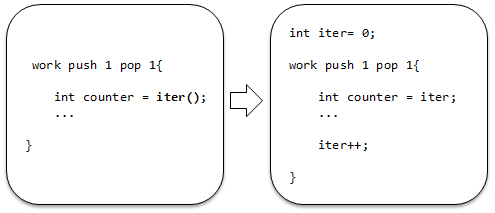
\includegraphics[width=3.3in]{figures/desugaring.png}
%\caption{Desugaring a filter using \texttt{iter()} keyword.\protect\label{fig:desugar}}
%\end{figure}


Under the StreamIt framework, filters are classified as iteration filters when there is use of the iteration keyword in its work function.  A simple lexer and parser can identify the use of this keyword, and it is represented accordingly in the intermediate representation.  To have it actually return the correct iteration value, we first convert the keyword to a compiler-usable construct.

{\tt iter()} is replaced with an access to a field holding the value of the iteration count.  The filter is given a definition for this field only if an {\tt iter()} use exists in its work or prework definition.  The work and prework function are appended with incrementing statements that update the iteration value.

The introduction of this iteration field creates state in the provided filter.  For future operations, the compiler does not consider this iteration field as part of the state of filter.  Future processes will maintain this inherent state without the downsides of introducing state.

It is important to note, these filters are not classified as stateful to the user, even though the filter is actually stateful on the iteration count after the desugaring process.  In classifying filters as stateful, the user is made aware of where data parallelism may be inhibited.  Iteration filters will not inhibit data parallelism because its state is identifiable to the compiler during the fission process.   


\section{Generalized Fission of Sliding Window Filters}
\label{sec:fission}

This section provides an overview of our technique for the fission of
sliding window filters. A complete description is given in
Figure~\ref{fig:general-fission} in the Appendix.  Our technique for
filter fission employs an optimization termed {\it synchronization
  removal}.  This transformation is applied to nodes calculating the
identity function in the general graph such that they can be removed,
but their communication patterns remain embedded in the general
graph. A description of synchronization removal is beyond the scope of
this paper, for a complete exposition, please see~\cite{mgordon-phd}.

The fission transformation applied to $f$ by factor $P$ divides $f$'s
work among $P$ fission products: $f_1...f_P$.  After the
transformation, each $f$ performs $M(S,f) /P$ iterations of $f$'s work
function in the steady-state.  The work of $f$ in the initialization
stage is preserved and translated to $f_1$.  The following
preconditions must be met before it $f$ can be fissed by $P$:
\begin{enumerate}
\item Fission products divide the work of $f$ evenly:
{\ninepoint
\begin{equation}
M(S,f) \mod P = 0 
\label{eq:mod-fiss}
\end{equation}
}
\item The items remaining in the input buffer of the original filter
  after initialization must be less than the number of items that will
  be dequeued by each fission product:
{\ninepoint
\begin{equation}
C(f) < (M(S,f) / P) \cdot o(W, f)
\label{eq:fiss-precond1}
\end{equation}
}
\end{enumerate}

\noindent The second precondition assures that no item is read by more
than 2 fission products.  As Section~\ref{sec:data-par} describes,
both of these preconditions can be enforced on any filter by
increasing the steady-state of the graph.  Fission includes the
following steps: 
\begin{enumerate}
\item Create $P$ copies of $f$ and set their rates
and work functions according to Figure~\ref{fig:general-fission}.
\item Create two identity nodes, $ID_I$ and $ID_O$, that will encode
  the distribution for the fission.
\item Move the initialization stage computation of $f$ to $f_1$
  according to Figure~\ref{fig:general-fission}. 
\item Move input distribution of $f$ to $ID_I$
replacing occurrences of $f$ with $ID_I$ in edges.
\item Move output distribution of $f$ to $ID_O$, replacing
occurrences of $f$ with $ID_O$ in edges.
\item Create the fission duplication pattern in the
output distribution of $ID_I$.
\item Create a round robin joining pattern for the output identity
  filter $ID_O$ to receive from each fission product.
\item For each node $p$ that is a producer of $f$, replace the
 occurrences of $f$ with $O_I$ in the edges of the dupsets of $p$'s
 output distribution.
\item For each node $c$ that is a consumer of $f$, replace the
 occurrences of $f$ with $O_O$ in incoming edges $c$'s input
 distribution.
\item \textsc{SynchRemove}($ID_I$)
\item \textsc{SynchRemove}($ID_O$)
\end{enumerate}

The details of fission on a filter of the general stream graph are
given in the Appendix in Figure~\ref{fig:general-fission}: (a) the
definition of the original filter $f$, (b) the steps of the algorithm,
and (c) details for steps 1-9.

\begin{figure*}
\centering
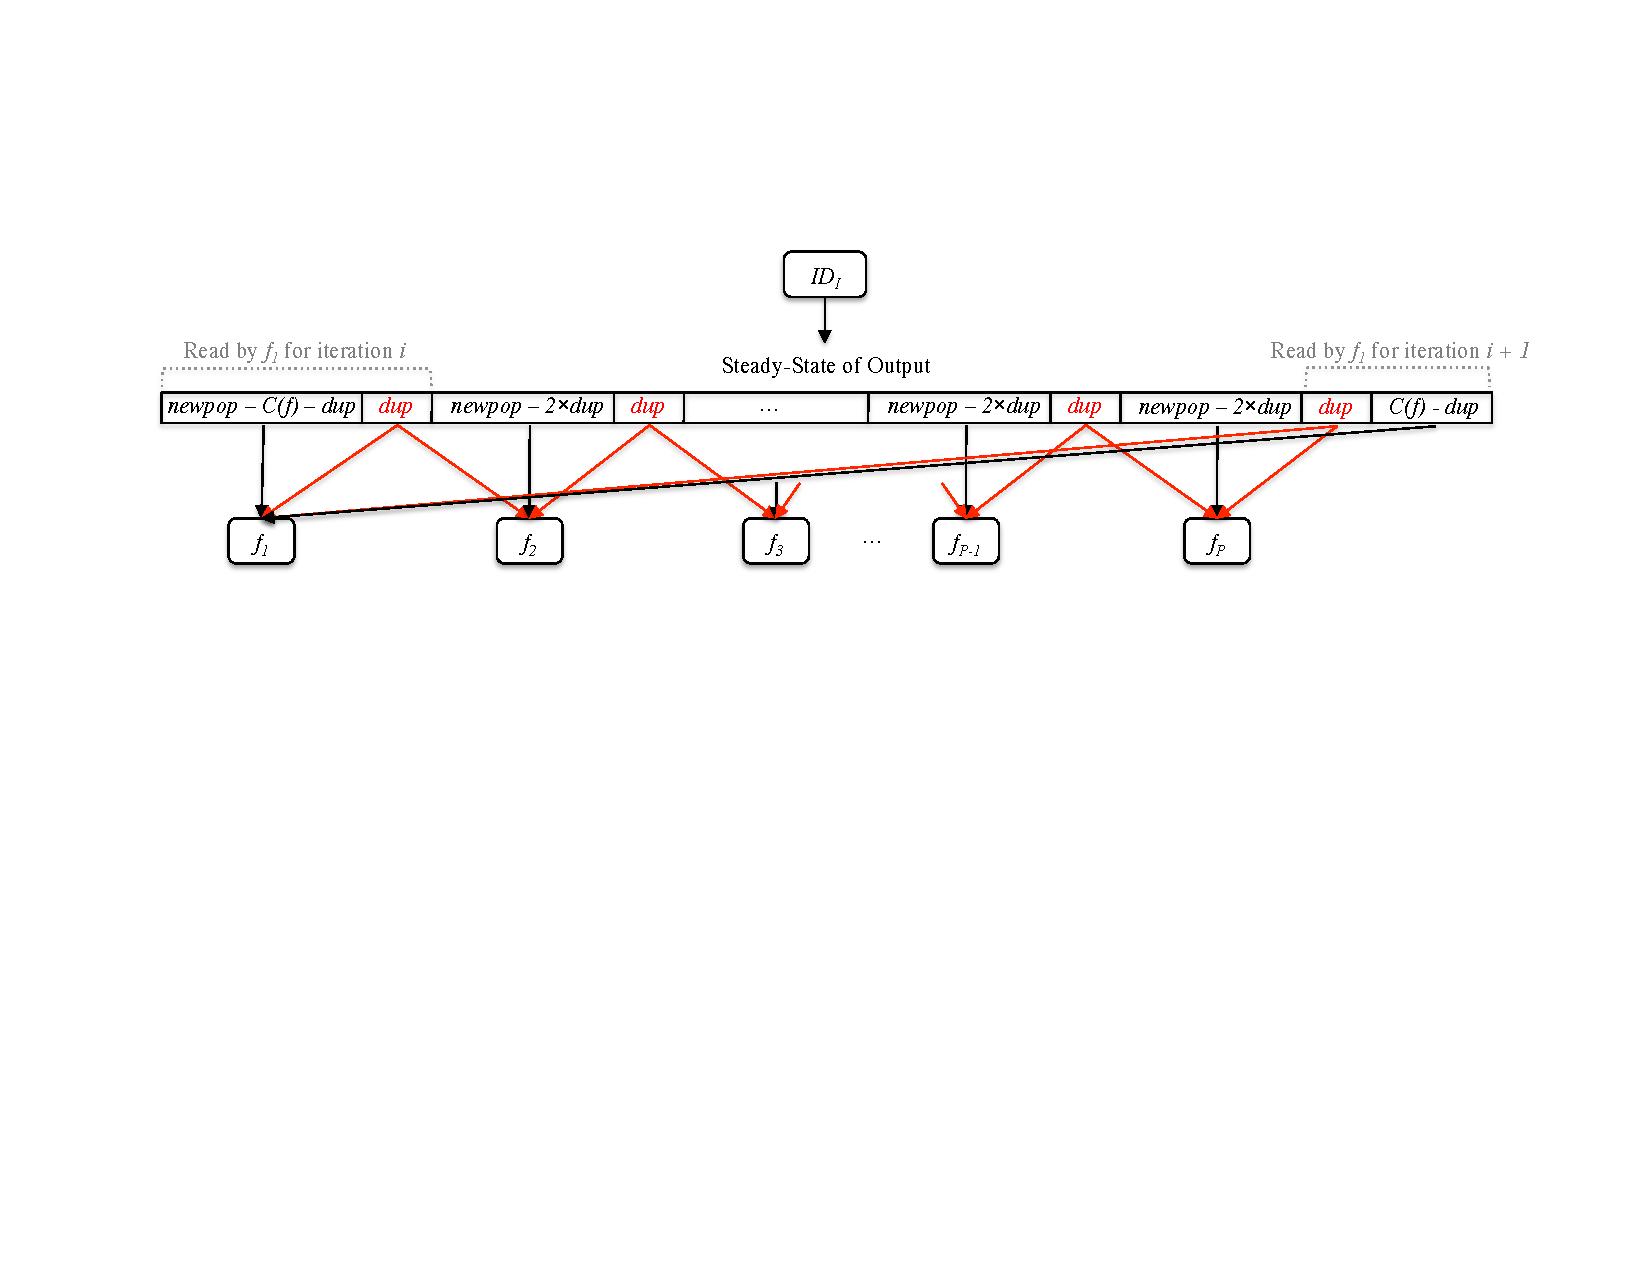
\includegraphics[width=6.3in]{figures/split-pattern.pdf}
\caption[The output distribution required for general
fission.]{
The steady-state output distribution installed for identity node
$ID_I$ by general fission.  Red edges denote items that are shared
across fission products via duplication. If $C(f) > dup$, $C(f) - dup$ items at the end of the
steady-state input are distributed to
$f_1$. \label{fig:split-pattern}}
\vspace{-10pt}
\end{figure*}

The general fission transformation creates two identity nodes ($ID_I$
and $ID_O$) that are encoded to implement the data distribution for
the fission products.  Figure~\ref{fig:split-pattern} illustrates the
pattern of communication between $ID_I$ and the products of $f$.  This
pattern is common to the transformation for all filters we seek to
fiss that meet the preconditions of the transformation.

The fission transformation has the following properties:
\begin{itemize}
\item No item is read by more than 2 fission products.
\item A fission product does not need to remember items across
  steady-state executions of itself. The peeking of the original
  filter $f$ is now encoded in the sharing across fission products
  achieved via the duplication pattern.
\item Only the first fission product $f_1$ is required to receive the $C(f)$
  initialization  items because $C(F) < (M(S,f) / p) \cdot o(W, f)$,
  and it will consume the $C(f)$ items on its first invocation.
\item The presence of the $C(f)$ items in the input buffer after
  initialization must be accounted for by shifting the read pattern
  for the fission products.  The first fission product $f_1$ is offset by
  $C(f)$ items in that it reads its first $C(f)$ items from the
  previous execution stage.  In the steady-state, $f_1$ executing at
  steady-state iteration $i$ shares items with $f_P$ executing at
  steady-state iteration $i-1$.
\item The computation and communication performed by $f$ during the
  initialization stage is transferred completely to the first fission
  product, $f_1$.  
% Since, by construction, only $f_1$ requires the
%   items remaining after the initialization stage.  The other fission
%   products are idle during this stage.
\end{itemize}

% The final steps of the general fission transformation applies
% \textsc{SynchRemove} to remove the identity filters, and stitch the
% communication directly between the fission products and $f$'s
% producer(s) and consumer(s).
 


% To understand the transformation, we first need to understand the item
% distribution and sharing that is required by fission on a filter $f$
% that adheres to the preconditions above.
% Figure~\ref{fig:fission-sharing2} gives another example of the input
% items required by fission products.  In this example, both:

% \[ C(f) = \mt{dup}_f < (M(S,f) / p) \cdot o(W, f) \]
% \[ M(S, f) \mod P = 0\]

% \noindent so $f$ adheres to the preconditions stipulated above for
% general fission.  In the example, the items read for $f$ plus its
% fission products for $P=4$ are shown for the initialization plus two
% steady-states.  After the initialization stage, $C(f) = 2$ items are
% enqueued to the input buffer by the producer(s) to $f$, and $M(S,f)
% \cdot o(W, f) = 16$ items are enqueued by the producer(s) for each
% steady-state.  Examining the sharing requirement for fission products of
% the second steady-state, we can see a pattern emerge with the following
% features:
\section{Analysis}

\begin{figure}[t]
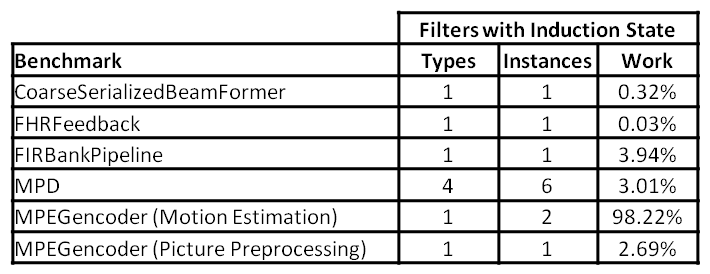
\includegraphics[width=3.5in]{figures/induction-benchmarks.png}
\caption{Benchmarks using induction variable state and estimations on work performed in filters with induction state.\protect\label{fig:benchmarks}}
\end{figure}

Figure~\ref{fig:benchmarks} indicates programs in the StreamIt benchmark suite that use induction variable filters (not including source filters).  The StreamIt compiler provides static estimations of work performed in filters.  The above table indicates the work performed in specifically the induction variable filters.

The majority of programs do not have substantial work performed in filters using induction variables, the MPEG-2 motion estimation subset being the exception.  However, eliminating state will have a large impact on runtime performance even on programs with low work concentration in stateful filters.  We model the potential speedups of a particular stateful program in this section.  For the purpose of this analysis, we will assume no communication cost between filters.  We will also assume the compiler exposes no pipeline parallelism.  This assumption forces the serialization of stateful filters on the stream graph.

Let $N$ be the number of cores we are planning to parallelize over.  Let $\sigma$ be the percentage of work performed in stateful filters that can have its state eliminated, in this case solely filters that use induction variable state.  

If $\sigma = 0$, the entire program is stateless.  The program can be fused to coarsen the granularity, then fissed and mapped to all of the available cores.  Each core would perform $\frac{1}{N}$ of the total work.  Thus with no state, the program can exhibit speedups of up to $N$ times the single-core runtime.

For filters that contain stateful work, we describe the program in terms of work that can be parallelized with work that cannot be parallelized.  $1-\sigma$ of the work in the program is considered stateless, and thus can be fissed and assigned to $N$ individual cores.  The stateful filters cannot be parallelized, and is sequential to all work in the program.  The total serialized work is $\frac{1-\sigma}{N} + \sigma$.  Thus the total speedup is the amount of work done without parallelization, or 100\% of the work, divided by the new parallelized work.  
\begin{eqnarray*}
\dfrac{1}{\frac{1-\sigma}{N} + \sigma} &=& \dfrac{N}{1 + \sigma(N-1)}
\end{eqnarray*}

We can characterize the amount of speedup between a completely stateless program to an equivalent stateful program with $\sigma$ percentage of stateful work.  This is simply:
\begin{eqnarray*}
\dfrac{N}{\frac{N}{1 + \sigma(N-1)}} &=& 1 + \sigma(N-1)
\end{eqnarray*}



\begin{figure}[t]
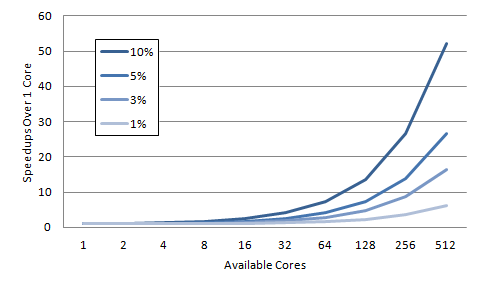
\includegraphics[width=3.5in]{figures/theoretical-speedups.png}
\caption{Theoretical speedups for stateless filters over corresponding stateful filters with $\sigma$\% work.  \protect\label{fig:theo-speedups}}
\end{figure}

Figure~\ref{fig:theo-speedups} indicates the potential speedups over stateful programs given stateful work percentages and a varying number of cores.  Even benchmarks in the suite that exhibit only 3\% work in stateful filters can exhibit 8x speedups with 256 cores.  Providing a means to remove state from filters that exhibit very small amounts of work relative to the rest of the program can still generate substantial speedups in the near future.



\begin{figure}[t]
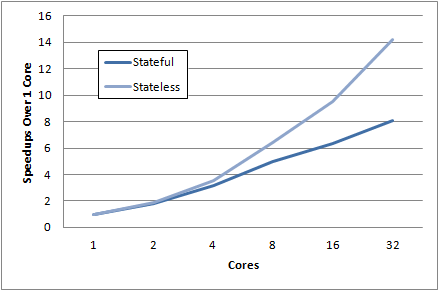
\includegraphics[width=3.5in]{figures/firbank-results.png}
\caption{Speedups for FIRBankPipeline, with and without induction variable state.  \protect\label{fig:firbank-results}}
\end{figure}

FIRBankPipeline contains one filter that uses induction variable state.  According to Figure~\ref{fig:benchmarks}, there is 3.94\% of work performed in the induction filter, which represents the only state in this benchmark.  Figure~\ref{fig:firbank-results} indicates the speedups over 1 core for both stateful and stateless implementations.  Between stateful and stateless implementations, there is 1.35X speedup on 8 cores, 1.58X speedup on 16 cores, and 1.84X speedup on 32 cores, which abides fairly closely to the model.
\section{MPEG-2 Motion Estimation Subset}


\begin{figure}[t]
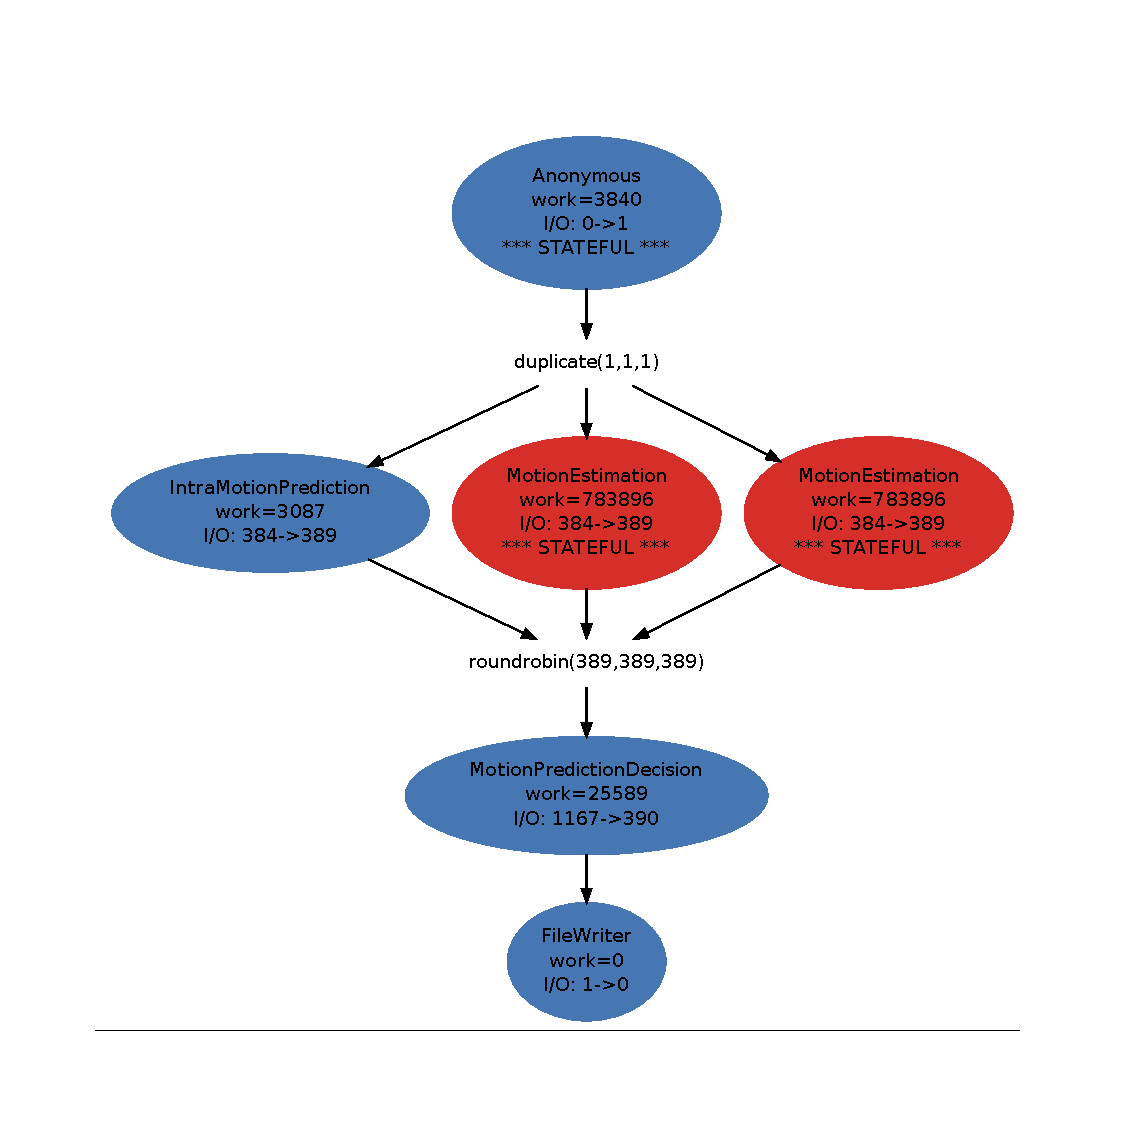
\includegraphics[width=3.5in]{work_estimate_mpeg_motionestimation.pdf}
\caption{MPEG Motion Estimation stream graph.\protect\label{fig:mpegMEgraph}}
\end{figure}


This section presents an application of induction variables to the Motion Estimation compression subset of the MPEG-2 encoder.  MPEG-2 is a standard for coding moving pictures and audio information and has a wide variety of multimedia applications.  

The specification contains various types of compression, one of which is motion prediction.  Motion prediction is a lossless compression, or one that eliminates redundant information from a signal while allowing for an exact reconstruction.  Motion prediction takes advantage of the fact that frames of a video contain a large amount of temporal redundancy.  A particular video sequence often contains duplicated scenes between consecutive frames.  Motion estimation attempts to generate motion predictions with respect to a set of reference frames.  These reference frames can be obtained from previous pictures or from both previous and future pictures.  Accordingly, the MPEG-2 encoder can utilize forward and backward motion estimation to achieve this form of compression.

The MPEG-2 standard organizes pictures into 16x16 groups of pixels called macroblocks.  Each macroblock is itself comprised of four 8x8 blocks of pixels termed as blocks.  Macroblocks can be encoded without any motion prediction, known as intra coded pictures, with only forward motion prediction, known as predictive coded pictures, and with both forward and backward motion prediction, known as bidirectionally predictive coded pictures.  These macroblocks are the basis of MPEG-2 motion prediction.  

The process of Motion Estimation entails comparing macroblocks between frames.  The motion estimator forms a motion vector that indicates a cartesian displacement of the macroblock from the most similar macroblock in the reference frames.  The matching macroblock is also removed from the new macroblock, yielding a residual macroblock that contains the difference between the prediction and the actual macroblock being encoded.  

The Motion estimation stream subgraph of the MPEG-2 encoder is illustrated in Figure~ref{mpegMEgraph}.  Each macroblock will be tested against all three types of prediction (intra coded, forward predicted, and backward predicted) to determine which is the best method for motion estimation.  The MotionEstimationDecision filter determines of these results, which is the best encoding technique.

[cite madrake meng 06]

The work estimation of this compression indicates the filter MotionEstimation is stateful and contains the majority of the work.  The duplicate splitjoin sends a copy of the picture to both forward and backward MotionEstimation and IntraMotionPrediction.  

The MotionEstimation filter pulls macroblocks at a time, iterating through a two-dimensional array (16x16 macroblocks) along the picture.  The filter relies on induction variables to maintain its array position.  We can apply the induction variable transformation on this filter to remove the state in the filter.

Reference pictures are set using upstream messaging from later in the stream graph.  Currently the backend does not support the use of upstream messaging, so for the purpose of benchmarking this application, the reference picture is set to a dummy value and is unchanged throughout the program.  This does not detract from the data parallelism introduced after removing the induction state.  Upstream messaging would simply require that sent messages be duplicated to all fissed filters in the stream graph.

Figure~ref{} shows the runtime figures for the original stateful MPEG-2 motion estimation subset compared to the stateless subset.  We can see significant improvements to runtime after making this subset stateless.  
\section{Related Work}
\label{sec:related}

These capabilities enable a programmer to write an application and its
filters at a natural granularity that is independent of
parallelization considerations enabling portable, reusable, and
malleable code.  Furthermore, fine-grained implementations of filters
enables the compiler to perform guided filter fusion that balances
data and instruction cache behavior~\cite{sermulins-lctes05}.


Need to address the coarsening issue.  Brook, which disallows state
would force the user to just coarsen the filter.  Why wouldn't someone
just coarsen?  


\section{Conclusions and Future Work}
\label{sec:conclusion}

This paper makes two contributions.  First, it introduces teleport
messaging: a powerful language construct enabling precise message
delivery between nodes of a distributed stream program.  In comparison
with other methods to implement messaging functionality in a
Synchronous Dataflow (SDF) model, teleport messaging is arguably more
readable, more robust, and easier to maintain.  In addition, our
implementation of teleport messaging in the StreamIt compiler resulted
in a 49\% performance improvement for a frequency hopping radio
running on a cluster of workstations.  Like several declarative
language constructs, teleport messaging improves performance by
exposing the true dependences to the compiler and allowing it to
optimize the communication.

%% We outlined several possible applications of $\sdep$, including
%% latency constraints, debugging, speculation, and program analysis, and
%% we look forward to pursuing these directions in the future.

Second, this paper formulates $\sdep$, a natural and useful dependence
representation for the streaming domain.  While this paper applies
$\sdep$ to a new language construct, we envision other applications as
well.  For example, $\sdep$ could be used in a debugger to identify
which iterations of an upstream actor are affecting a given iteration
of a downstream actor.  In a software-based speculation
system~\cite{frank-thesis}, $\sdep$ could be applied to trace the
effects of a failed prediction and to roll back the appropriate actor
executions.  $\sdep$ also offers a new method for measuring latency in
a stream graph.  Similar to representations such as dependence
levels~~\cite{AK82}, direction vectors~\cite{wolfe82}, and dependence
polyhedra~\cite{Irig88} for scientific programs, $\sdep$ provides
dependence information that could be used to test or verify program
transformations.

There are some limitations in the current study that are fertile
grounds for future research.  First, our formulation of $\sdep$
requires a directed path in the stream graph (aligned with the
direction of data flow) between the actors in question.  We are
generalizing $\sdep$ to actors that run in parallel by leveraging
their data dependences with common predecessors (upstream) or
successors (downstream).  Second, as detailed in
Section~\ref{sec:constraints}, we do not solve the general scheduling
problem that incorporates overlapping constraints from teleport
messaging; even determining whether or not a set of constraints is
feasible (especially during the initialization
schedule~\cite{karczma-thesis}) seems to be an interesting question.
Third, in the current model only actors can send and receive messages.
We are extending this into a hierarchical model where stream
containers (such as pipelines) can also receive events and dispatch
them precisely to other streams.  Finally, our approach relies on the
static communication rates present in SDF.  It would be interesting to
consider teleport messaging in a more dynamic context; for example,
downstream non-negative latency messages could be immediately
supported by embedding messages in data items, while other messages
might require speculative delivery or modified timing contracts.

Our work can be viewed as the integration of dynamic behavior into a
static dataflow language.  Our insight is that there is a class of
control messages that only adjust a parameter in the target actor;
they do not otherwise affect the input or output channels upon
delivery.  This model enables a hybrid scheduling scheme in which the
steady-state dataflow is exactly orchestrated at compile time, but
there are windows in which a message could adjust an internal field of
an actor between its execution steps.  We consider this to be a
promising avenue for creating a unified development environment that
captures all aspects of stream application development without
sacrificing either performance or programmability.


% \acks
% Acknowledgments, if needed.

% We recommend abbrvnat bibliography style.
\ninepoint
\bibliographystyle{abbrvnat}
\bibliography{references}


\end{document}

